\documentclass[12pt,a4paper]{report}
\usepackage{amsmath,amsthm,amssymb,graphicx,hyperref}
\usepackage[left=1.2in,right=1in,top=1in,bottom=1in]{geometry}
\usepackage[romanian]{babel}
\usepackage{hyperref}
\usepackage{subcaption}
\usepackage{titlesec}
\usepackage{float}
\usepackage{listings}
\newcommand{\sectionbreak}{\clearpage}

\begin{document}
\thispagestyle{empty}
\begin{center}
\begin{figure}[h!]
\vspace{-20pt}
\begin{center}

\includegraphics[width=100pt]{FMI-03.png}
\end{center}
\end{figure}


{\large{\bf UNIVERSITATEA DE VEST DIN TIMI\c SOARA

FACULTATEA DE MATEMATIC\u A \c SI INFORMATIC\u A

PROGRAMUL DE STUDII DE LICEN\c T\u A: INFORMATIC\u A APLICAT\u A }}

\vspace{120pt}
{\huge {\bf LUCRARE DE LICEN\c T\u A}}

\vspace{150pt}
\end{center}

{\large\noindent{\bf COORDONATOR:\hfill ABSOLVENT:}

\noindent Conf. Dr. Fortiș Teodor-Florin \hfill Kiss Flavia-Maria}

\vfill
\begin{center}
{\bf TIMI\c SOARA

2021}
\end{center}
\newpage
\thispagestyle{empty}
\begin{center}
{\large{\bf UNIVERSITATEA DE VEST DIN TIMI\c SOARA

FACULTATEA DE MATEMATIC\u A \c SI INFORMATIC\u A


PROGRAMUL DE STUDII DE LICEN\c T\u A: INFORMATIC\u A APLICAT\u A }}

\vspace{120pt}
{\huge {\bf PROACTIV}}

\vspace{150pt}
\end{center}

{\large\noindent{\bf COORDONATOR:\hfill ABSOLVENT:}

\noindent Conf. Dr. Fortiș Teodor-Florin \hfill Kiss Flavia-Maria}

\vfill
\begin{center}
{\bf TIMI\c SOARA

2021}
\end{center}
\newpage
\normalsize{}

\setcounter{page}{2}

\section*{Abstract}
\par
"Proactiv" is a web platform focused on volunteering. Through it, potential volunteers can get in touch with different organizations or companies, and organizations can post their own volunteer activities and find the volunteers they need to successfully accomplish its organization and development.
\\ \par
The site has a friendly interface, with a pleasant design, it's easy to navigate and has as main element the Google Map, a map on which volunteer activities are listed as pins, depending on the location where they take place. 
\\ \par
I chose this name because the term “proactivity” is quite often used in IT companies and is an encouraged and appreciated skill in the workplace. I consider a proactive person to be dynamic, involved, willing to try new things and, most importantly, focused on innovation and evolution.


\section*{Rezumat}
\par
Platforma “Proactiv” este o platformă web axată pe tema voluntariatului. Prin intermediul acesteia, posibilii voluntari pot lua legătura cu diferite organizații sau
firme, iar organizațiile pot semnala acțiunile de voluntariat proprii și pot găsi voluntarii de care au nevoie în îndeplinirea cu succes a acesteia.
\\ \par
Site-ul are o interfață prietenoasă, cu un design plăcut, ușor de navigat și are ca element principal harta celor de la Google, hartă pe care sunt semnalate acțiunile de voluntariat sub forma unor pini, în funcție de locația la care acestea se desfășoară.
\\ \par
Am ales acest nume deoarece termenul de “proactivitate” este destul de des folosit în companiile din domeniul IT și este o competență încurajată și apreciată la locul de muncă. Consider o persoana proactivă ca fiind dinamică, implicată, dispusă să încerce lucruri noi și, cel mai important, axată pe inovare și evoluție.

\tableofcontents
\newpage

\chapter{Introducere}
\section{Descrierea problemei}
\par
Precum este menționat pe site-ul hipo.ro\cite{proactiv}, deși este un termen des folosit în literatura de management și în jargonul de resurse umane, nu se găsește termenul de “proactivitate” în dicționar. Înțelesul lui ar putea fi rezumat într-o accepțiune limitată la a lua inițiativa. Într-un context mai larg, a fi proactiv înseamnă a-ți asuma responsabilitatea lucrurilor care ți se întamplă și a înceta să dai vina pe ceea ce este în jurul tău pentru faptul că anumite lucruri nu se întamplă sau se mișcă foarte greu. 
\\ \par
“Proactiv” este o platfomă web axată pe tema voluntariatului, care pune în legătură posibili voluntari cu diferite organizații sau firme care caută acest lucru. Utilizatorii au posibilitatea de a-și creea un cont de tip voluntar sau de tip organizație/firmă. În funcție de tipul contului aceștia pot să caute sau să semnaleze o acțiune de voluntariat. Decizia de a crea această aplicație a pornit din dorința de a încuraja mai mulți oameni în a fi proactivi și implicați în societatea în care trăiesc. 
\\ \par
Mulți dintre noi suntem familiarizați cu conceptul de “voluntariat”. Acesta implică acțiuni efectuate din liber arbitru, în beneficiul comunității, nu cu scopul principal de a câștiga financiar. În esență, reprezintă decizia de ne oferi timpul și abilitățile pentru a aduce beneficii celorlalți.
\\ \par
Există un motiv pentru care voluntariatul a devenit atât de popular. În mod ideal, o experiență de voluntariat implică un schimb - de cultură, abilități, umanitate sau puncte de vedere - astfel încât fiecare parte să beneficieze. Acesta reflectă nevoia noastră umană de a ne conecta unii cu alții, de a învăța lucruri noi, de a contribui în societate sau de a ne oferi un scop mai mare vieții noastre: să ne înțelegem pe noi înșine, lumea și locul nostru în aceasta totodată.
\newpage
Voluntariatul are o mulțime de beneficii, precum consolidarea încrederii, competenței, conexiunilor și comunității. Acestea sunt ilustrate în Figura 1.1, imagine oferită de către Volunteer Benevoles Canada\cite{VBC}.
\begin{figure}[H]
\centering
  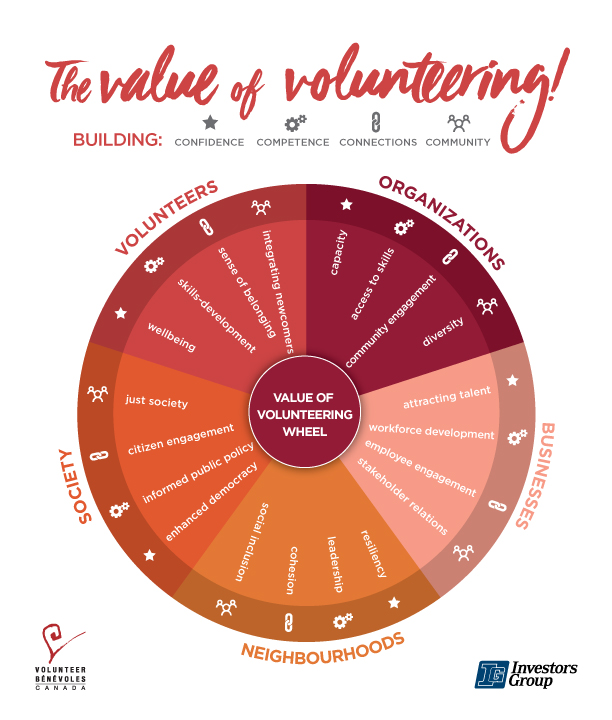
\includegraphics[width=0.7\linewidth]{./imagini/VC_ValueOfVolunteering.jpg}
  \caption{Roata Valorilor Voluntariatului}
\end{figure}

\par
Green Report\cite{greenr} ne relatează că doar trei români din zece fac voluntariat în mod activ pentru cauze sociale sau de mediu, fără a fi constrânși. Această informație reiese dintr-un studiu realizat de Hunters, o divizie de trenduri a companiei de cercetare Unlock Market Research.
\\ \par
Trebuie luat în considerare că există atât oameni care, deși și-ar dori să facă voluntariat și să ajute, nu știu unde să găsească oportunități, cât și organizații care sunt în căutare de voluntari. Scopul acestei platforme este acela de a rezolva această problemă și de a aduce mai aproape veștile și noutățile din acest domeniu de interes.
\\ \par
Aplicația “Proactiv” are o interfață prietenoasă, cu un design plăcut, ușor de navigat și, folosind Google Maps API, afișează pe harta României, sub forma unor pini, toate acțiunile de voluntariat active și semnalează utilizatorului posibilitățile acestuia în funcție de localizarea geografică. Pentru partea de frontend se folosesc HTML și CSS, pentru cea de backend JavaScript și PHP, iar pentru gestionarea bazelor de date MariaDB prin interfața PHPMyAdmin.

\section{Abordări existente și contribuții proprii}
\par
O abordare similară a problemei poate fi regasită pe “Harta Voluntariatului”\cite{hv}. Deși se poate observa că ideea de bază este una comună, designul și metoda de afișare a datelor diferă foarte mult. 
\\ \par
Precum se poate observa în Figura 1.2, pe platforma “Harta Voluntariatului” oportunitățile de voluntariat sunt trecute sub forma unui blog cu diferite articole, aparținând de diferite organizații. Pe acel site sunt afișate rezultatele în funcție de data la care începe proiectul, pe când “Proactiv” le afișează predominant în funcție de locația utilizatorului.
\begin{figure}[H]
\centering
  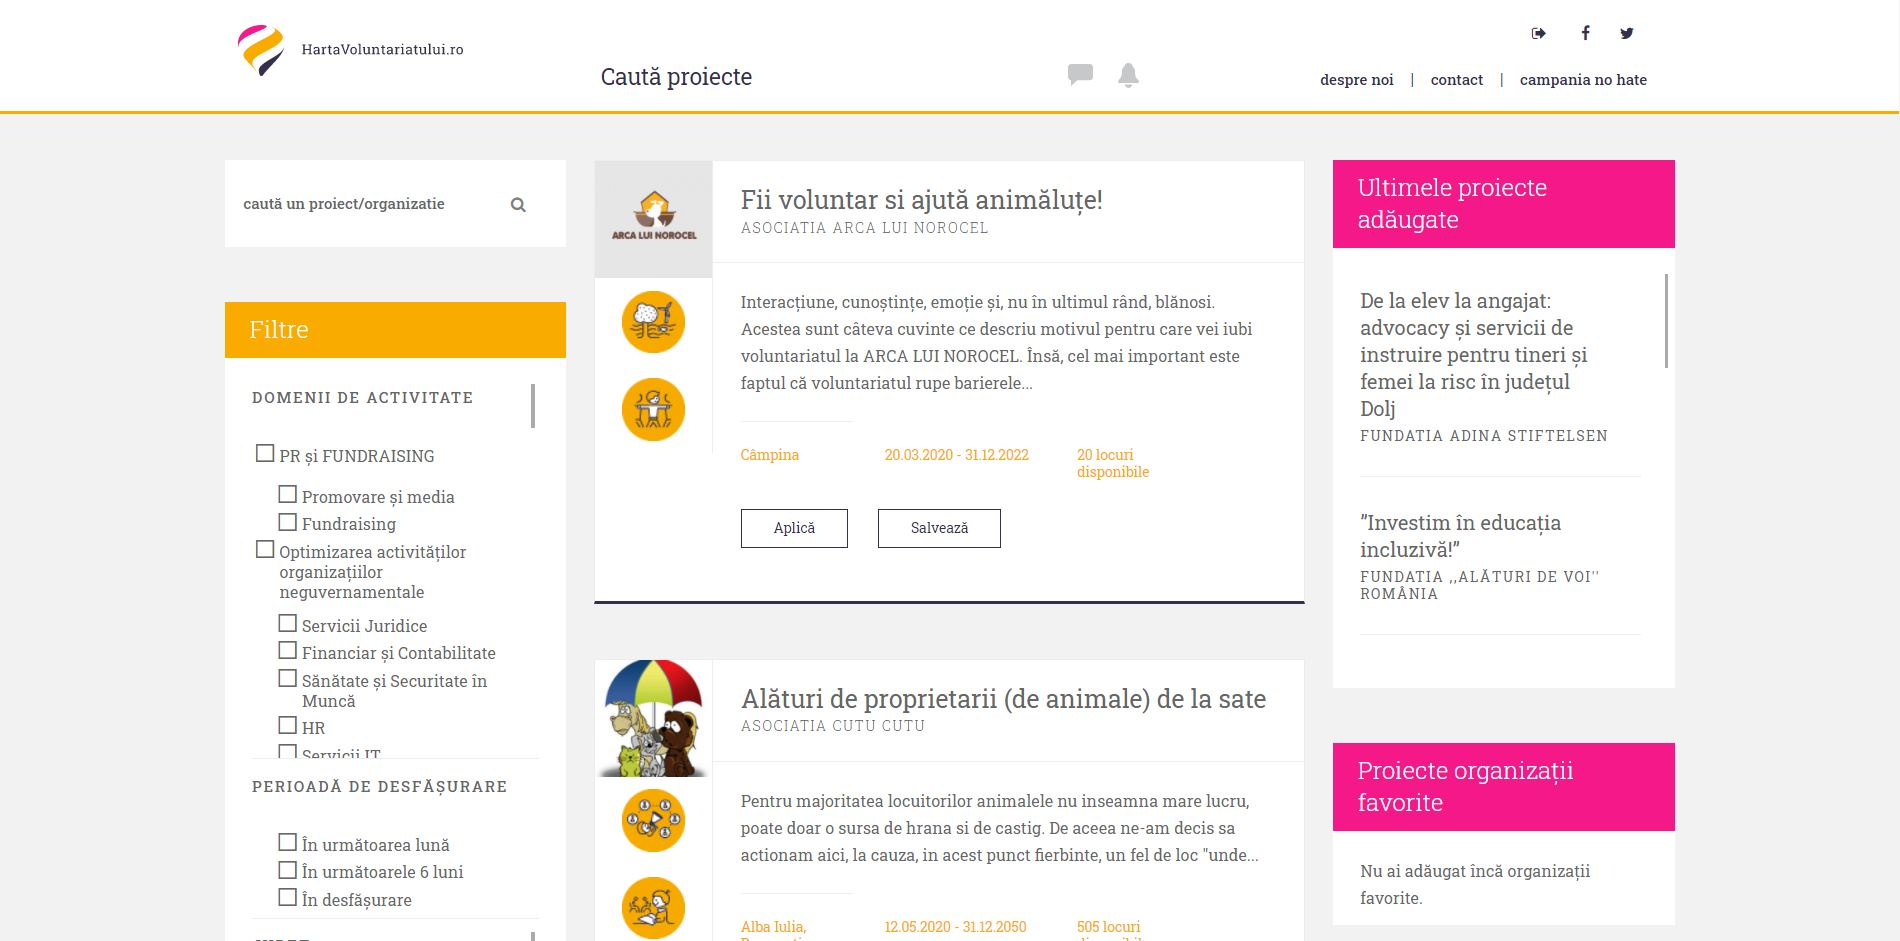
\includegraphics[width=1\linewidth]{./imagini/hv1.jpg}
  \caption{Secțiunea “Caută proiecte” a platformei Harta Voluntariatului}
\end{figure}

\newpage
Un alt site dedicat acțiunilor de voluntariat este “De Bunavoie”\cite{dbv}. Acesta are un design asemănător cu cel al platfomei “Harta Voluntariatului”, anume sub forma unui blog cu articole, pentru fiecare acțiune de voluntariat semnalată. Asemănarea dintre aceste două platforme poate fi observată comparând figura anterioară cu Figura 1.3 afișată mai jos.
\begin{figure}[H]
\centering
  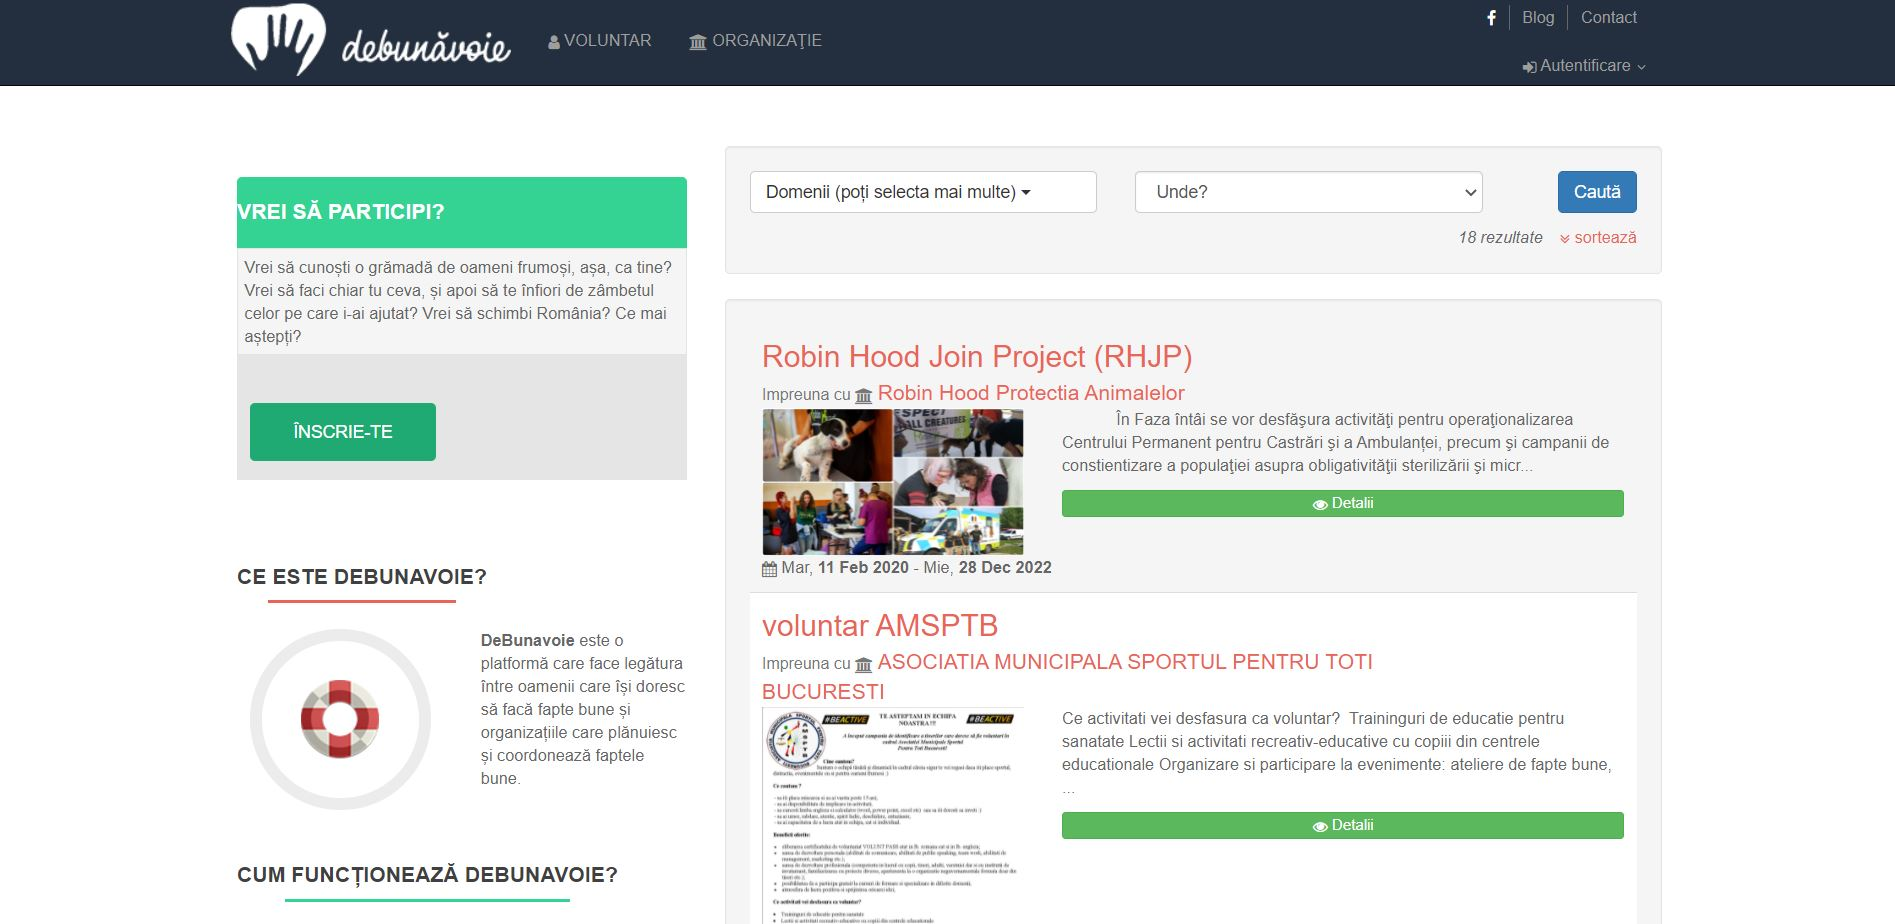
\includegraphics[width=1\linewidth]{./imagini/dbv1.jpg}
  \caption{Acțiunile semnalate pe platforma De Bunavoie}
\end{figure}

\par
Un avantaj al acestor site-uri este posibilitatea de a filtra domeniile de activitate, pentru a afișa utilizatorului doar proiectele din aria lui de interes. În acest fel, va crește eficiența căutării iar utilizatorul va fi mulțumit că a câștigat timp.
\\\par 
Un dezavantaj este metoda de prezentare a proiectelor, una obositoare ochiului. Fiind vorba despre platforme de tip blog, își fac apariția foarte multe descrieri și foarte mult text, acest lucru îngreunănd navigarea pe site și găsirea acțiunilor potrivite de către utilizatori. Comparativ cu acestea, platforma “Proactiv” prezintă acțiunile semnalate sub o formă cât mai simplă, vizuală și interactivă.
\newpage
De asemenea, există foarte multe platforme străine, destinate voluntariatului, precum “All For Good”\cite{afg}, prezentată în Figura 1.4, dar un mare dezavantaj al acestora este utilizarea limbii engleze și opțiunile limitate când este selectată România drept locație.
\begin{figure}[H]
\centering
  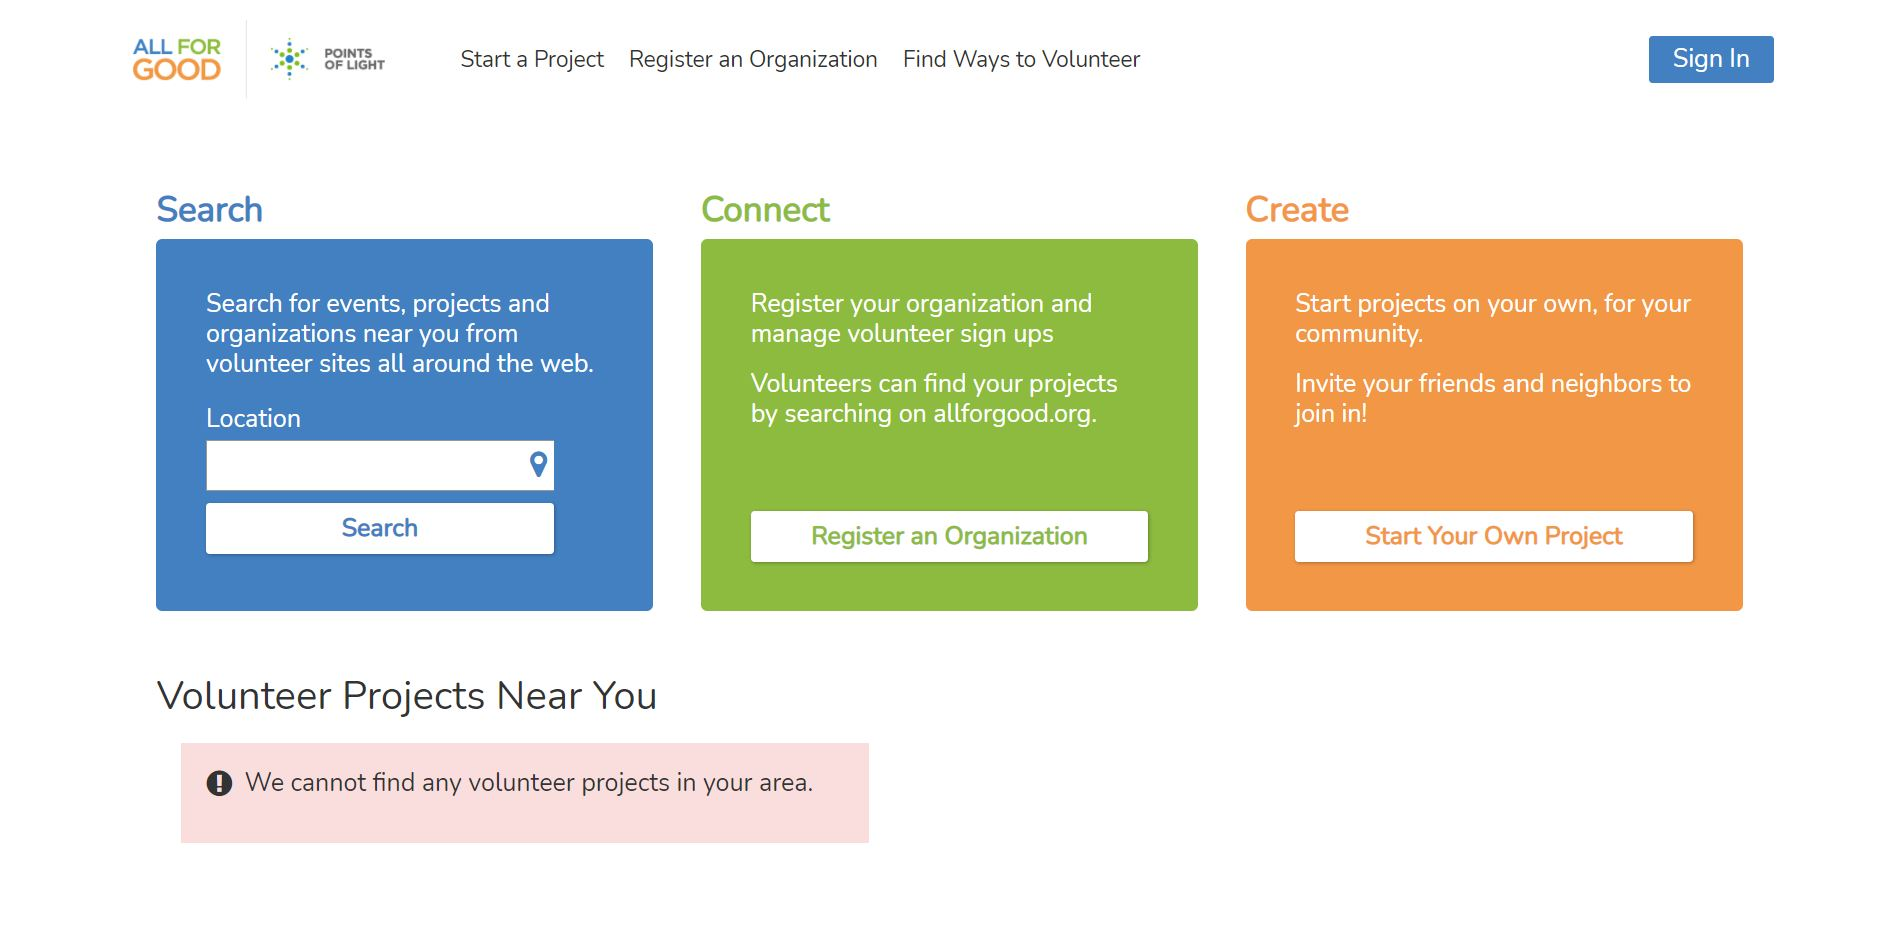
\includegraphics[width=1\linewidth]{./imagini/afg.jpg}
  \caption{Lipsa acțiunilor semnalate în zona României}
\end{figure}

\section{Organizarea lucrării}
\par
Tema generală a lucrării este voluntariatul, deoarece platforma “Proactiv” este dedicată acestui domeniu.
\\\par 
Lucrarea este organizată pe 5 capitole. În cadrul primului capitol am prezentat motivul alegerii numelui și a temei, beneficiile voluntariatului, platformele similare existente și diferențele dintre acestea și platforma mea, dar și contribuțiile proprii aduse acestei teme. În cadrul celui de al doilea capitol, am prezentat arhitectura aplicației, explicând și prezentând atât wireframe-ul platformei, cât și fiecare pagină web în parte.
\\\par 
Cel de-al treilea capitol se referă la funcționalitatea aplicației și cuprinde diagramele de cazuri, de secvențe, de activitate și de stări și tranziții. De asemenea, acest capitol conține informații despre fiecare funcționalitate a platformei și secvențe de cod referitoare la acestea.
\\\par 
Capitolul cu numărul patru prezintă structura bazei de date, fiind prezentate și ilustrate atât relația dintre tabele, cât și structura și conținutul fiecărui tabel în parte, iar ultimul capitol cuprinde concluziile și direcțiile viitoare de dezvoltare.


\chapter{Arhitectura aplicației}

\section{Introducere}
\par
Arhitectura site-ului web este structura ierarhică a paginilor acestuia. Această structură se reflectă prin legături interne și trebuie să îi ajute pe utilizatori să găsească cu ușurință informații. Arhitectura este foarte importantă în a face o primă impresie bună utilizatorului. Sunt studii făcute pe această temă, care ne relatează că aproape unul din doi utilizatori părăsesc un site încă de la prima pagină, cea principală.
\\\par 
Este critic ca un site web să aibă o structură intuitivă și ușor de navigat, pentru a păstra interesul utilizatorilor de a naviga în continuare.
\\\par 
Implementarea unei structuri ne ajută să proiectăm o platformă web cu o experiență plăcută pentru utilizator. Deși conținutul este, poate, unul uimitor, dacă utilizatorii nu îl pot găsi, aceștia vor pleca pe site-ul unui concurent.
\\\par 
O structură tipică arată ca un arbore, în care pagina principală este rădăcina. Paginile care sunt conectate din pagina de pornire sunt ramuri, iar de acolo, fiecare pagină are ramuri suplimentare care răsar din ea. Aceste ramuri se leagă apoi între ele, de obicei prin intermediul unui meniu.
\\\par 
Arhitectura platformei Proactiv poate fi regăsită în Figura 2.1. Pagina principală permite înregistrarea fie ca voluntar, fie ca organizație, sau autentificarea cu un cont deja existent în baza de date a platformei. După autentificare, tipul contului este recunoscut de către aplicație, aceasta redirecționând utilizatorul către conținutul potrivit nevoilor și dorințelor lui. Voluntarii au acces la harta Google Maps unde sunt semnalate acțiunile și la pagina care conține lista de organizații înscrise pe platformă, conturile de tip organizație au acces la pagina web care permite semnalarea unei acțiuni noi de voluntariat și la lista voluntarilor, iar ambele tipuri de cont au acces la pagina de acasă și la cea de gestionare a propriului cont.

\begin{figure}[H]
\centering
  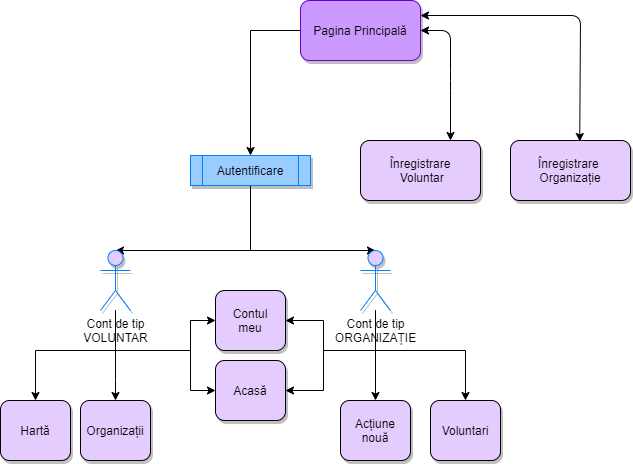
\includegraphics[width=1\linewidth]{./imagini/arhitectura.png}
  \caption{Arhitectura platformei Proactiv}
\end{figure}

\section{Wireframe}
\par
Wireframe-ul sau macheta funcțională este o diagramă utilizată în timpul proiectării unei interfețe utilizator pentru a defini zonele și componentele pe care aceasta trebuie să le conțină. Acesta descrie elementele de interfață, sistemele de navigație și modul în care acestea funcționează împreună.
\\\par
Un wireframe este un punct bun de pornire în realizarea interfeței în sine. Acesta este utilizat în principal în contextul dezvoltării site-urilor și aplicațiilor web. Structura acestuia constă în mod concret dintr-o schiță, un colaj de hârtie sau o diagramă digitală.
\\\par
În afara site-urilor web, machetele funcționale sunt utilizate pentru prototiparea site-urilor mobile, a aplicațiilor pentru computer sau a altor produse screen-based, care implică o interacțiune între om și computer.
\\\par
Wireframe-ul platformei Proactiv este ilustrat în Figura 2.2. Acesta a fost schițat înainte de a începe implementarea platformei, cu scopul de a vizualiza clar interfața acesteia și modul în care se dorește organizarea paginilor și poziționarea elementelor de front-end. 
Desigur, odată cu începerea implementării, și-au făcut apariția anumite modificări necesare în realizarea unei lucrări cu o arhitectură logică și intuitivă, dar proiectarea în sine a rămas aceeași.

\begin{figure}[H]
\centering
  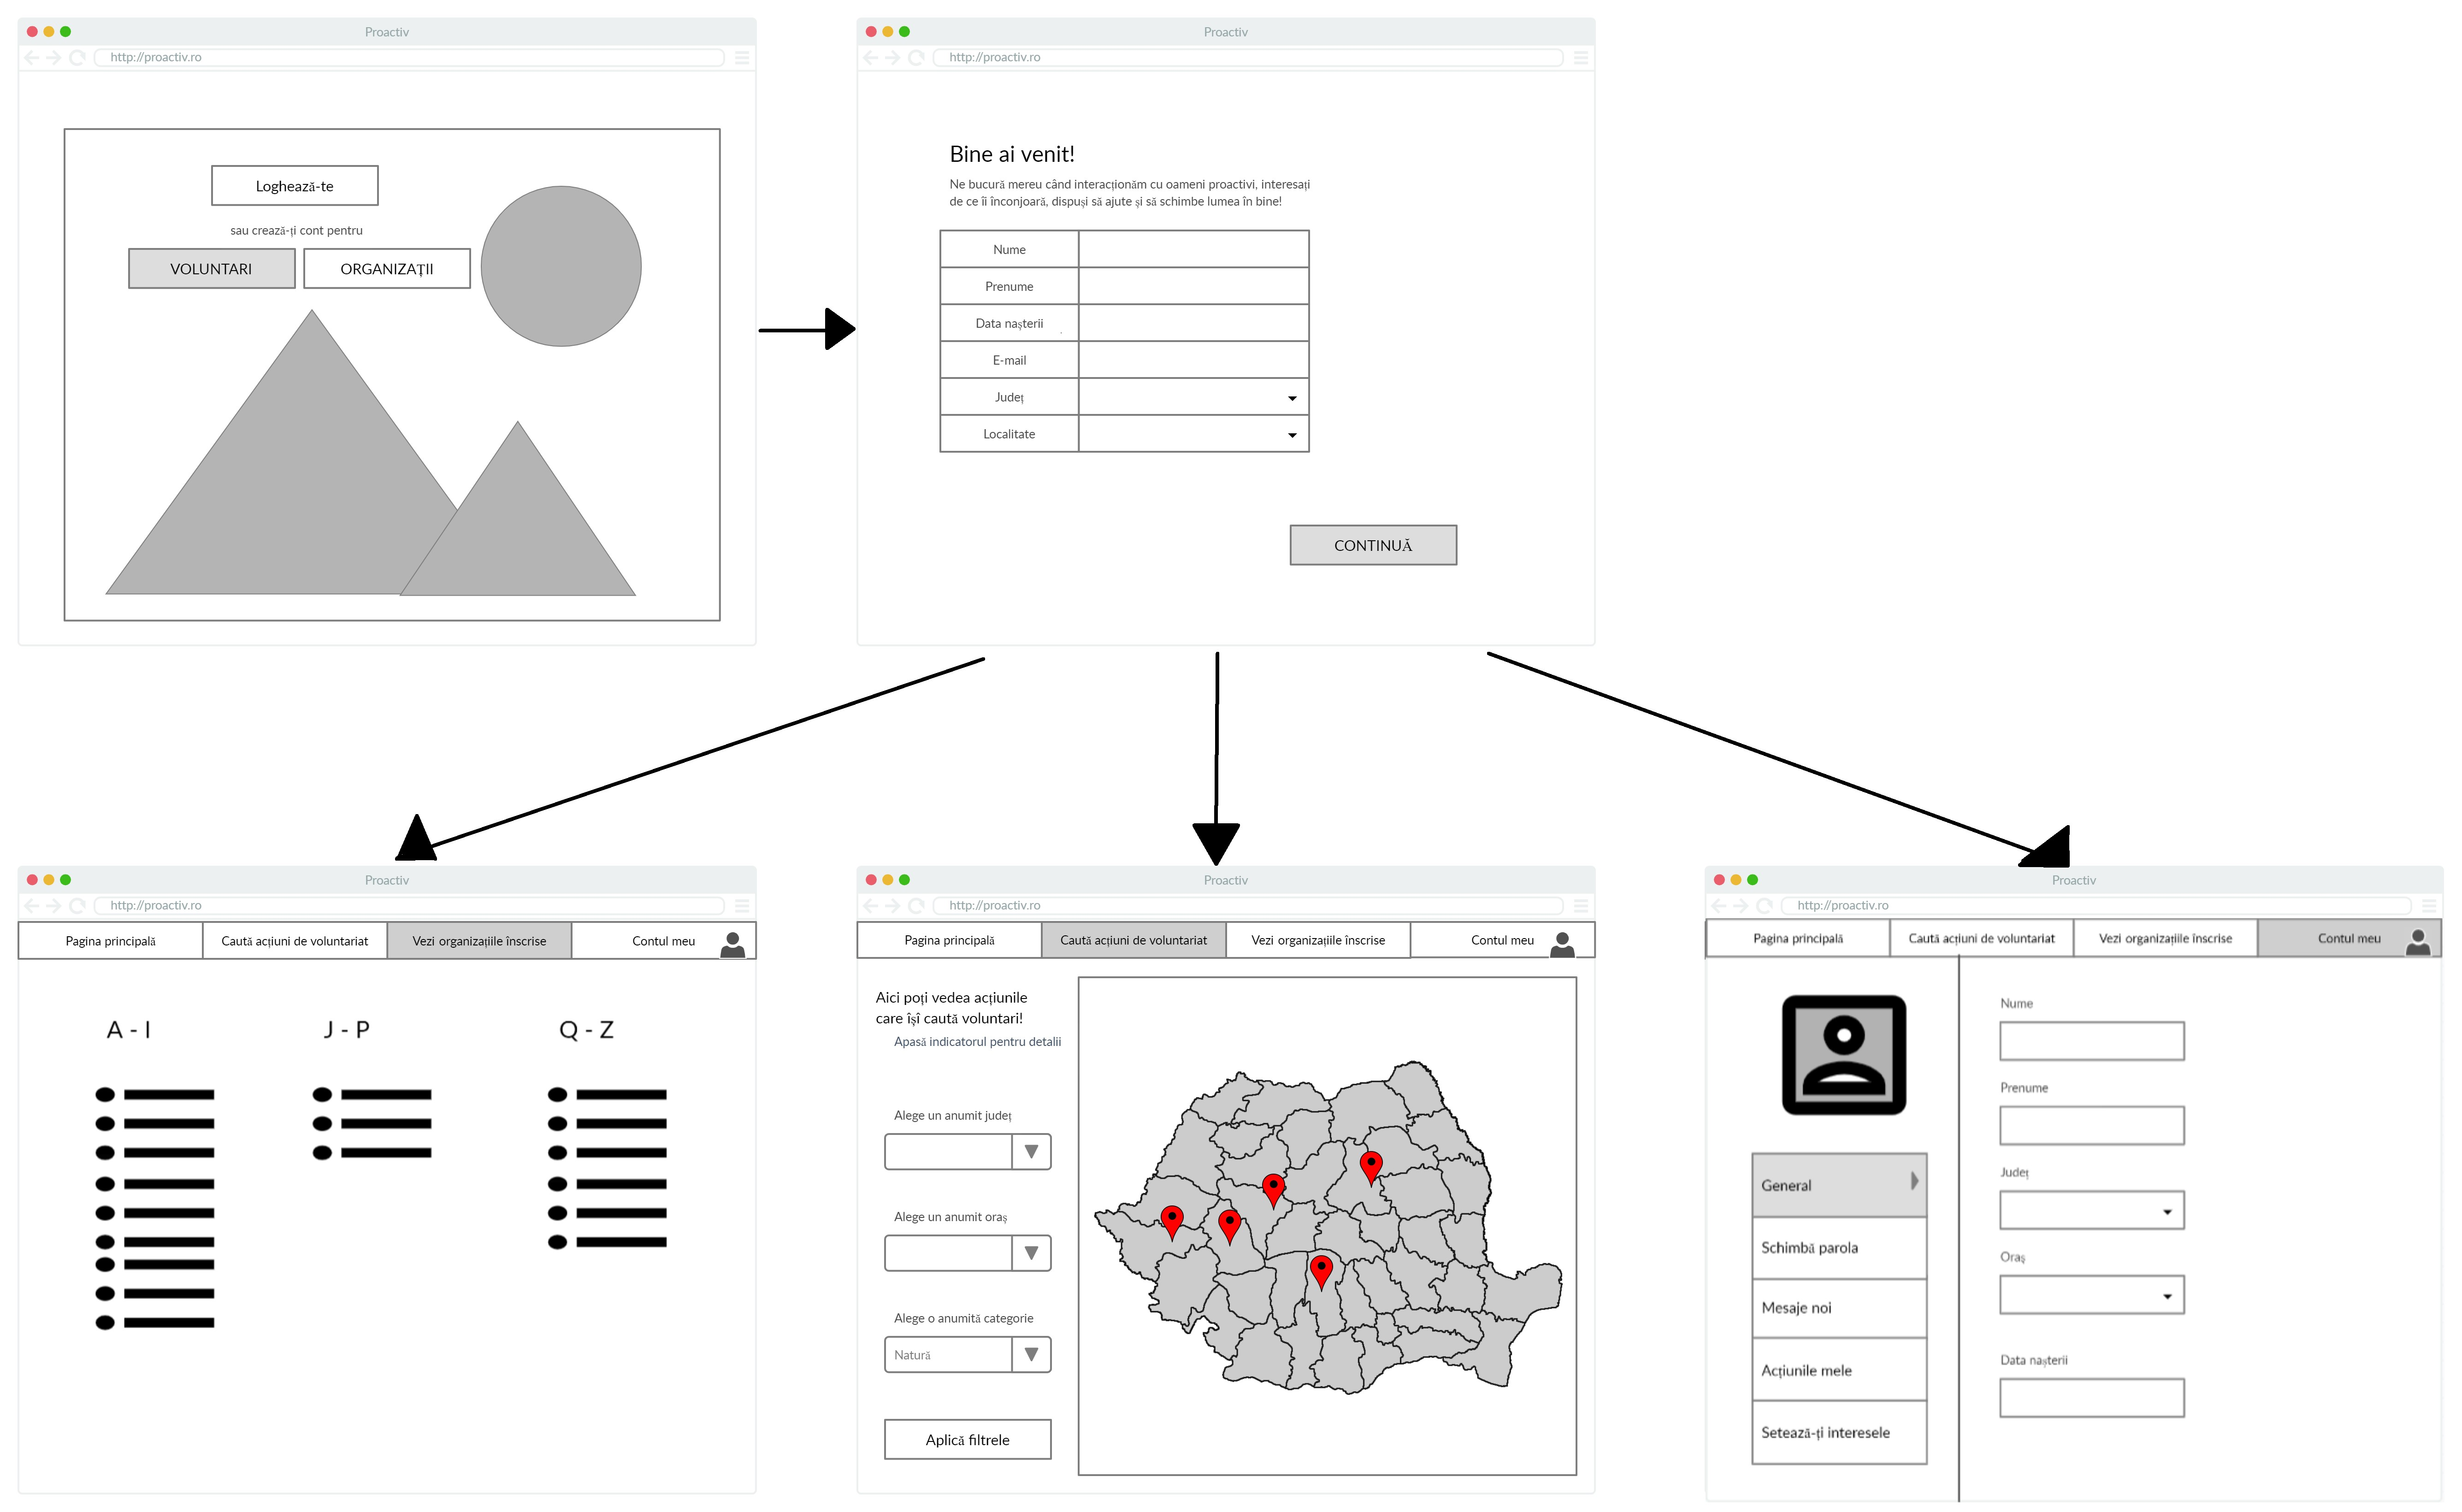
\includegraphics[width=1\linewidth]{./imagini/GUI.jpg}
  \caption{Wireframe-ul platformei Proactiv}
\end{figure}


\section{Pagina principală}
\par
Pagina principală este una dintre cele mai importante componente ale interfeței, deoarece este cea care întâmpină utilizatorul. Aceasta trebuie să îi capteze atenția și să îl convingă să navigheze platforma în continuare.
\\\par
Elementul dominant de pe pagina principală și, totodată, elementul pe care îl întâlnește utilizatorul în momentul accesării platformei Proactiv este caruselul (slideshow-ul) de poze, oferit de framework-ul Bootstrap. 
\\\par
Pagina principală cuprinde trei secțiuni, și anume:
\par

\begin{itemize}
  \item Partea de autentificare și de întâmpinare a utilizatorilor recurenți, ilustrată în Figura 2.3, care cuprinde o poză clară, atractivă și plăcută de către iubitorii de animale și un buton care deschide modalul de login - Figura 2.4, portal între pagina principală și paginile reprezentative site-ului meu de voluntariat.
\\
\begin{figure}[H]
\centering
  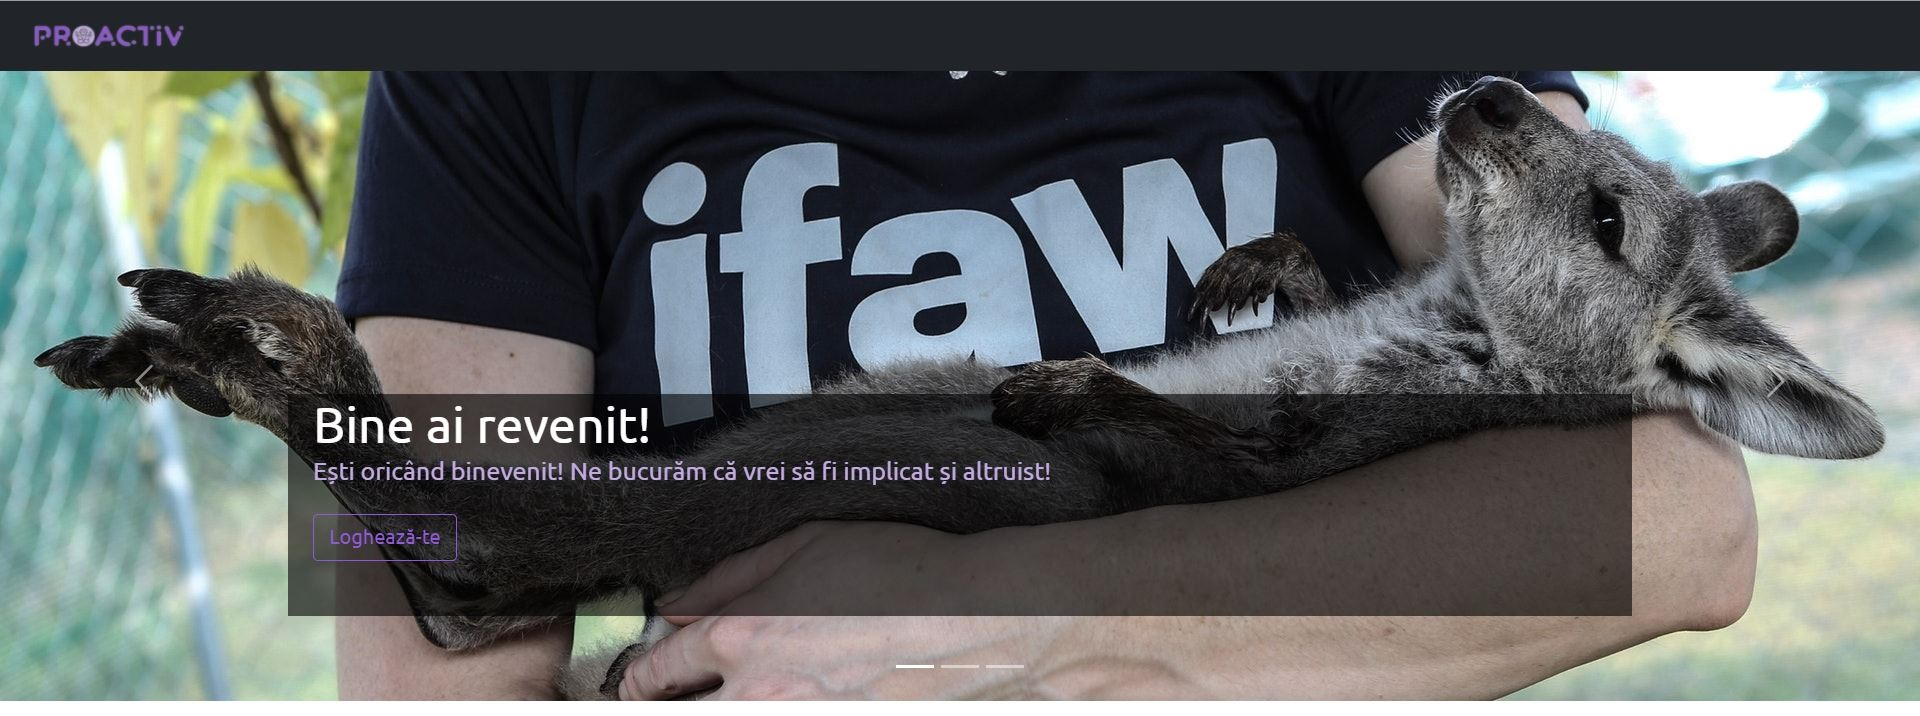
\includegraphics[width=1\linewidth]{./imagini/pp1.jpg}
  \caption{Secțiunea de autentificare a platformei Proactiv}
\end{figure}
\begin{figure}[H]
\centering
  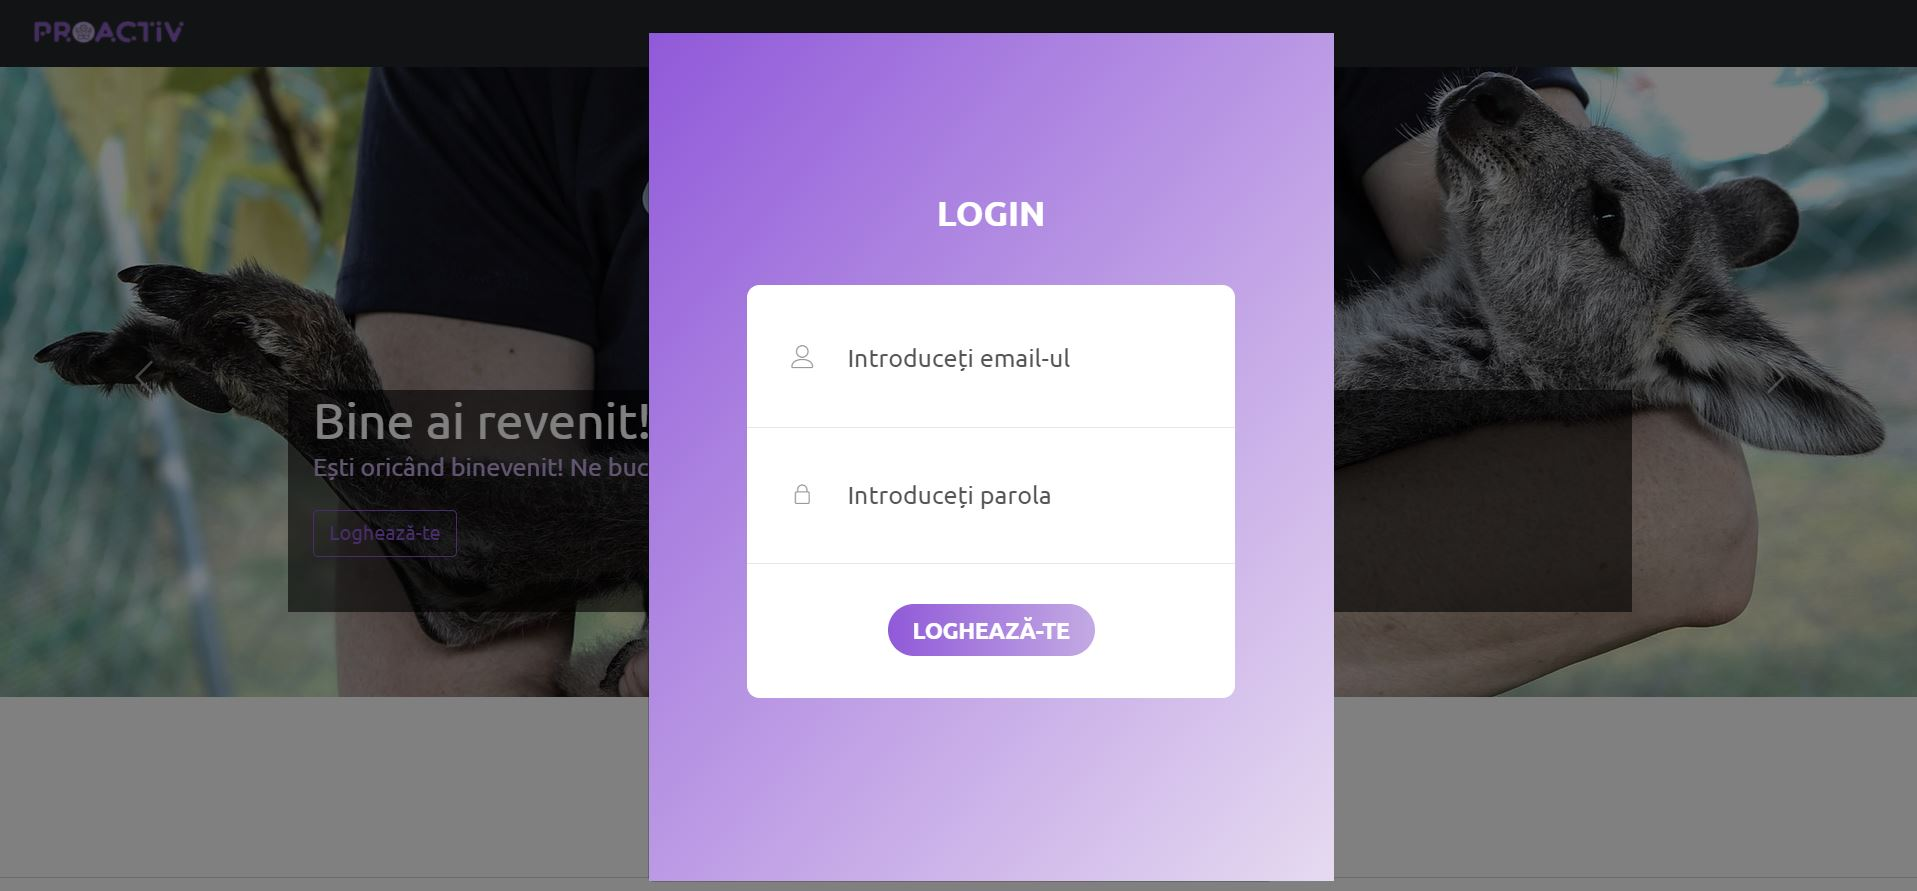
\includegraphics[width=1\linewidth]{./imagini/login.jpg}
  \caption{Modalul de login al platformei Proactiv}
\end{figure}
\newpage
  \item Partea de înregistrare - Figura 2.5, care încurajează utilizatorii noi să își creeze un cont și să se alăture platformei, șă fie proactivi. Pentru această secțiune am ales o poză cu un impact puternic, o poză “cât o mie de cuvinte”, pentru a atrage atenția utilizatorilor noi. Aici se regăsesc două butoane, unul pentru înregistrarea ca voluntar și altul pentru înregistrarea ca organizație. În funcție de butonul apăsat se va deschide pagina de “Cont nou Voluntar” sau cea de “Cont nou Organizație”.
\\
\begin{figure}[H]
\centering
  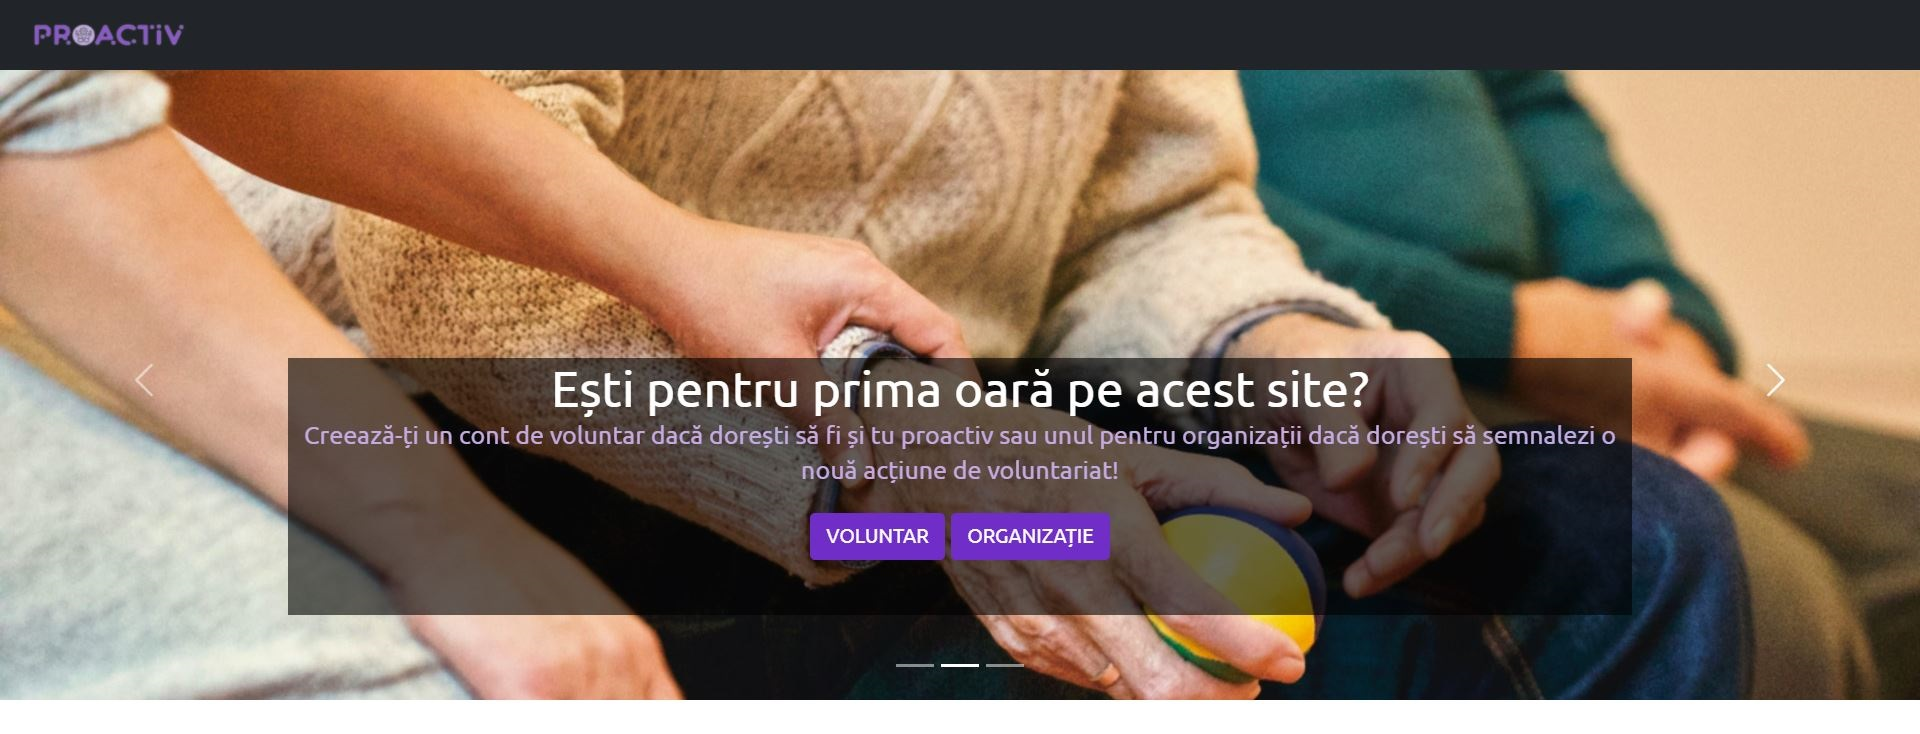
\includegraphics[width=1\linewidth]{./imagini/pp2.jpg}
  \caption{Secțiunea de înregistrare a platformei Proactiv}
\end{figure}
  \item Și secțiunea “De ce?” - Figura 2.6, pentru utilizatorii mai încăpățânați, pe care nu am reușit să îi conving să se alăture plaformei, dar cărora le mai este cerută o șansă, oferindu-le motive pentru care a face voluntariat este un lucru minunat.
\\
\begin{figure}[H]
\centering
  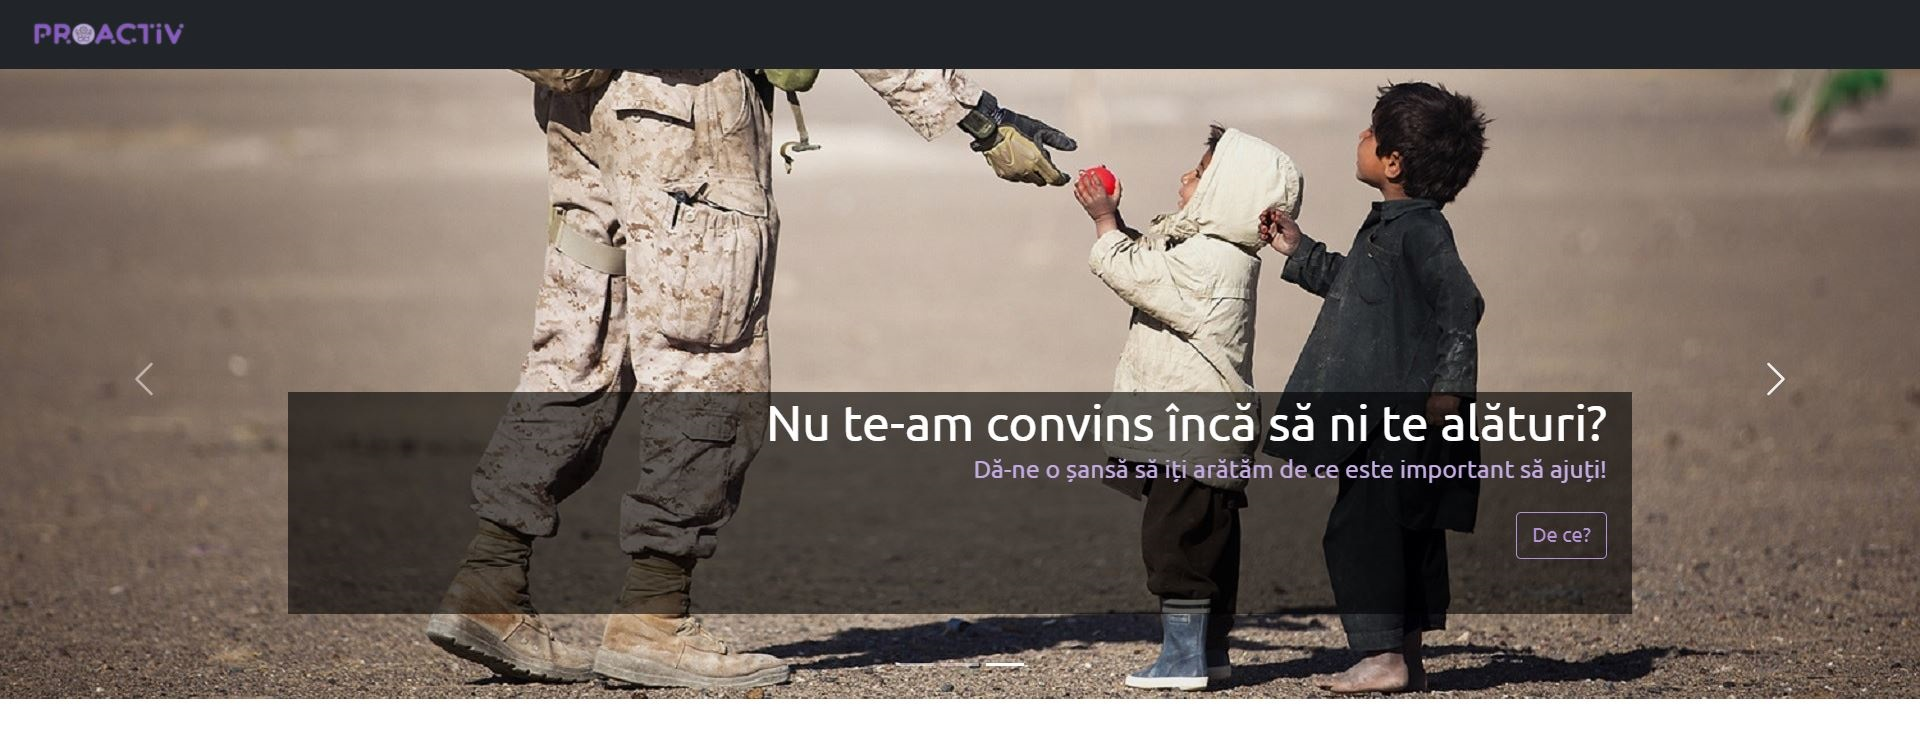
\includegraphics[width=1\linewidth]{./imagini/pp3.jpg}
  \caption{Secțiunea “De ce?” a platformei Proactiv}
\end{figure}
\newpage
În momentul apăsării butonului “De ce?”, pagina se va derula inferior caruselului de imagine și vor fi afișate pentru utilizator diferite motive pentru care merită să se alăture platformei și să fie proactiv. În momentul în care utilizatorul derulează până la limita inferioară a paginii, acesta are opțiunea de a se întoarce înapoi la slideshow, apăsând un hyperlink.
\\
\begin{figure}[H]
\centering
  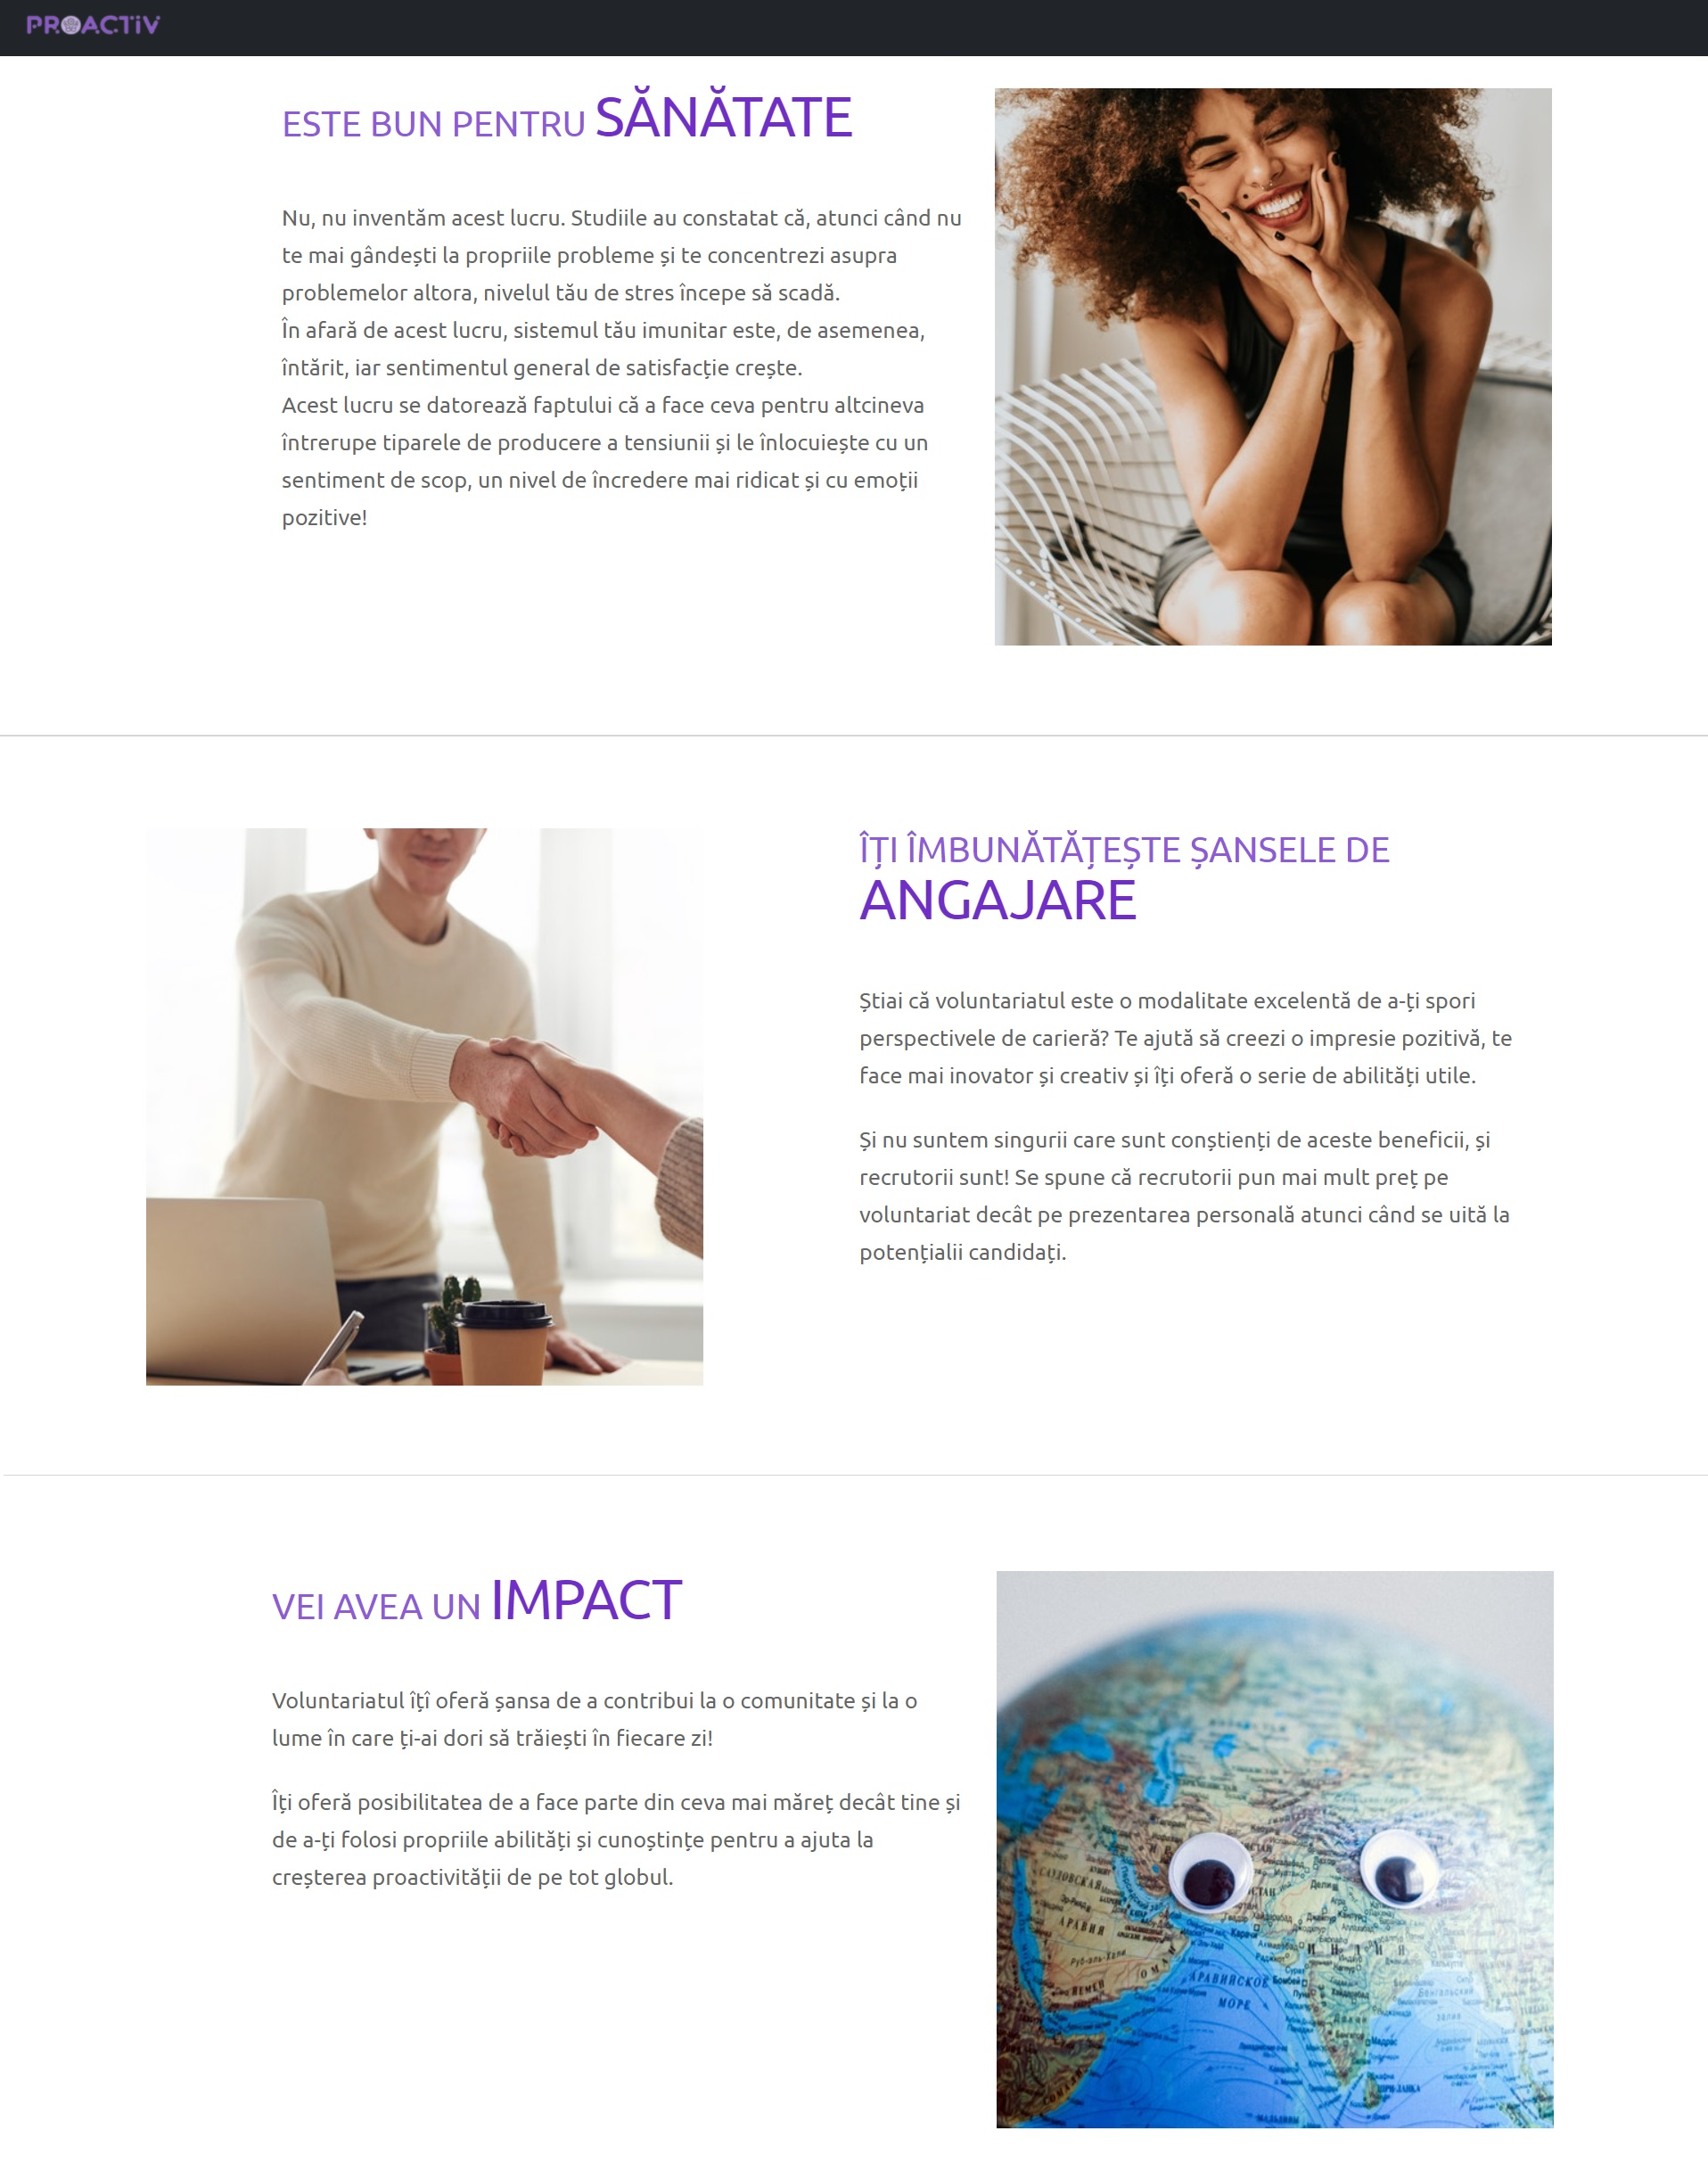
\includegraphics[width=1\linewidth]{./imagini/pp4.jpg}
  \caption{Motive temeinice pentru a face voluntariat}
\end{figure}
\end{itemize}

\section{Cont nou VOLUNTAR}
\par
Utilizatorul este redirecționat către pagina ilustrată în Figura 2.8 în momentul în care apasă butonul “Voluntar”, de la secțiunea de înregistrare a paginii principale.
\\\par
Pagina este un formular care cuprinde diferite tipuri de căsuțe de input, precum date-picker-ul de la “Data nașterii”, dropdown-ul de la “Județ”, cât și cel de la “Oraș”, care este dependent de primul, afișând doar orașele din județul ales anterior sau o listă goală în cazul în care nu a fost selectat nici un județ.
\\\par
În momentul apăsării butonului “Creează cont”, dacă toate datele corespund cerințelor, utilizatorul va fi redirecționat înapoi către pagina principală și se va putea autentifica cu credențialele proaspăt introduse.
\\\par
Pentru a reveni la pagina principală, în cazul în care utilizatorul decide să nu ducă la final înregistrarea, acesta poate apăsa sigla platformei din partea stângă a bării de navigare.
\\
\begin{figure}[H]
\centering
  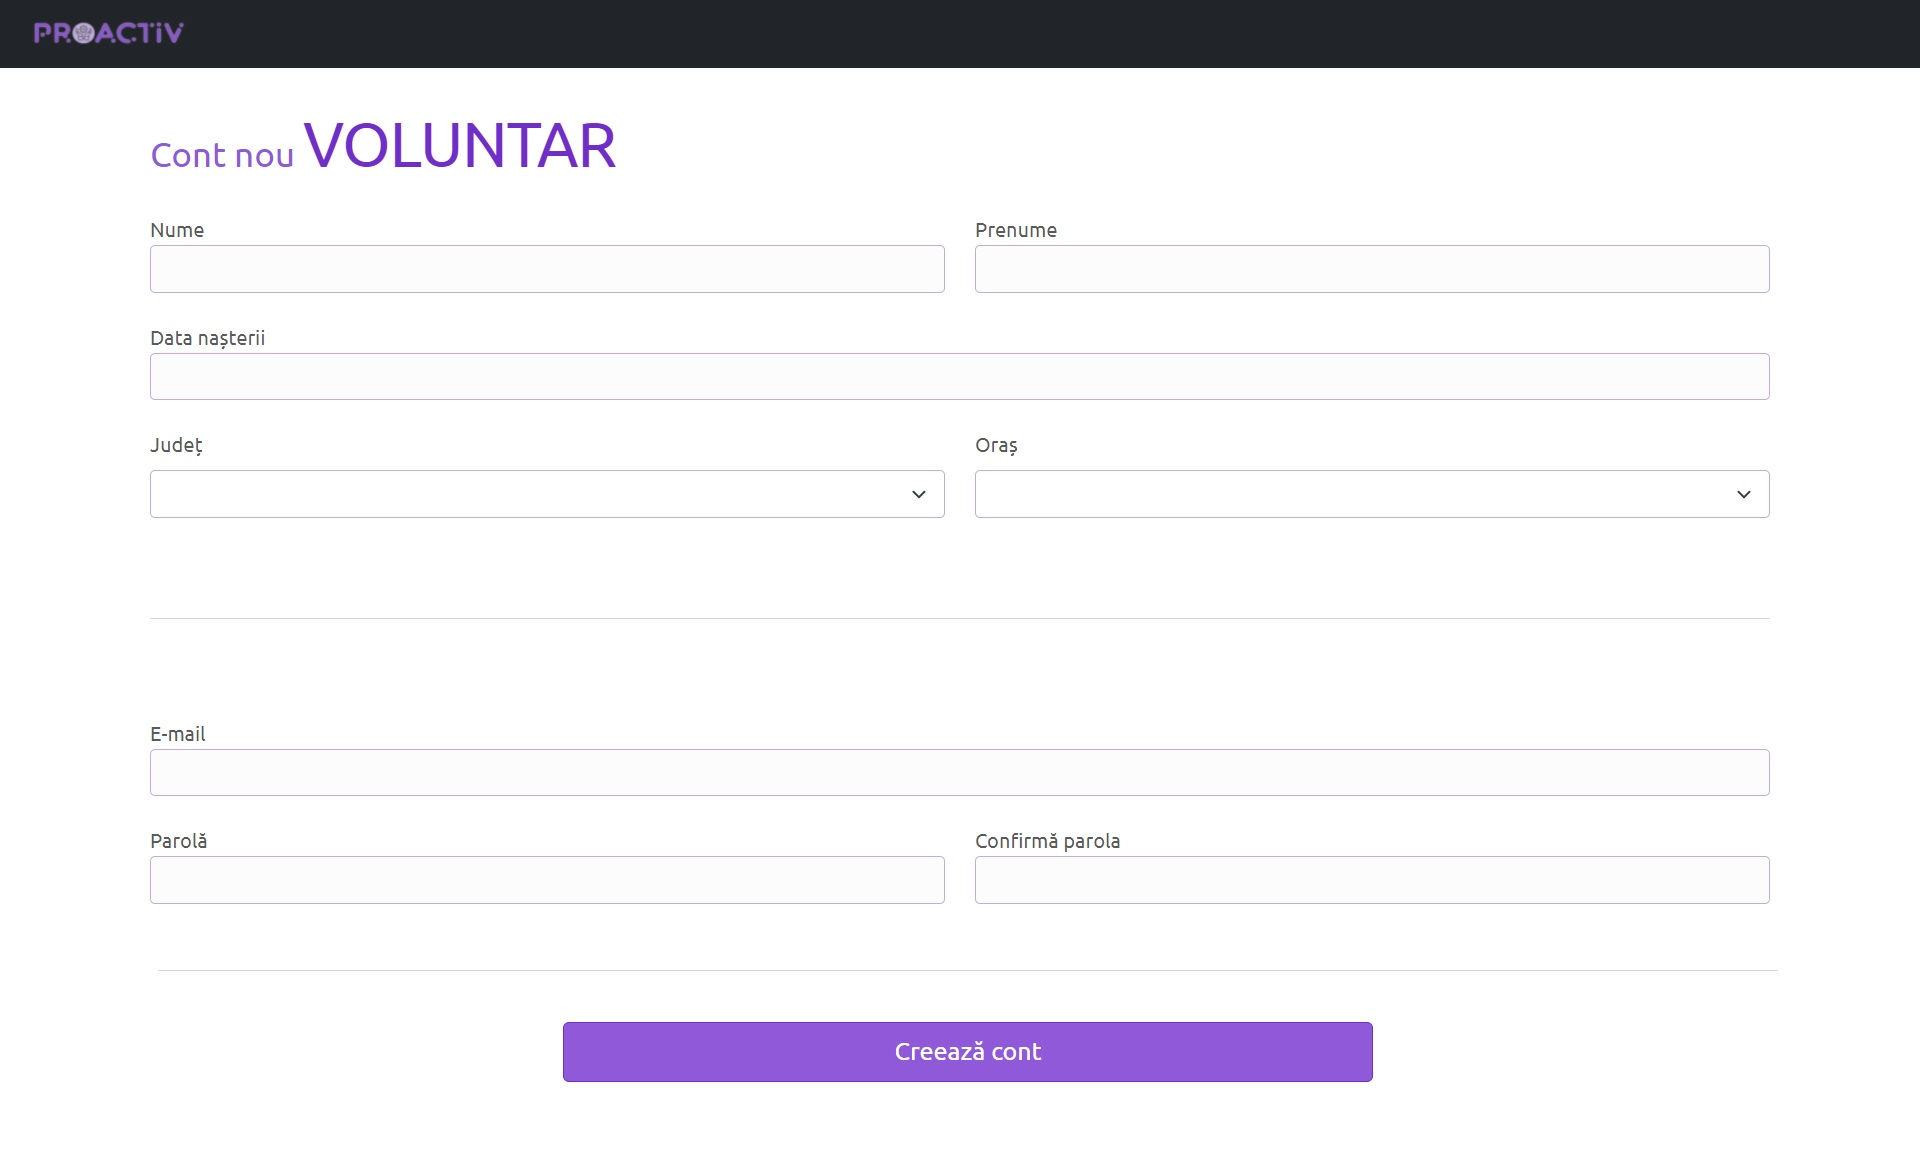
\includegraphics[width=1\linewidth]{./imagini/contvol.jpg}
  \caption{Pagina de înregistrare voluntar a platformei Proactiv}
\end{figure}

\section{Cont nou ORGANIZAȚIE}
\par
Precum se poate observa din Figura 2.9, această pagină este asemănătoare cu pagina aferentă înregistrării voluntarului.
\\\par
Sunt cerute anumite date personale reprezentative unei organizații, în locul datelor personale precum nume, prenume sau data nașterii. Pentru organizații, este necesară completarea tuturor câmpurilor: denumirea organizației, codul unic de identificare, data înfințării, județul și orașul unde își are reședința și o scurtă descriere despre organizație și activitatea pe care aceasta o desfășoară.
\\\par
Desigur, este necesară și completarea câmpurilor email și parolă, cu condiția ca emailul să aibă un format valid, să nu fie deja înregistrat pe platformă, iar ca parola și confirmarea acesteia să corespundă.
\\\par
În momentul apăsării butonului “Creează cont”, dacă toate datele sunt completate și corespund cerințelor, utilizatorul va fi redirecționat înapoi către pagina principală și se va putea autentifica cu credențialele contului tocmai înregistrat.
\\
\begin{figure}[H]
\centering
  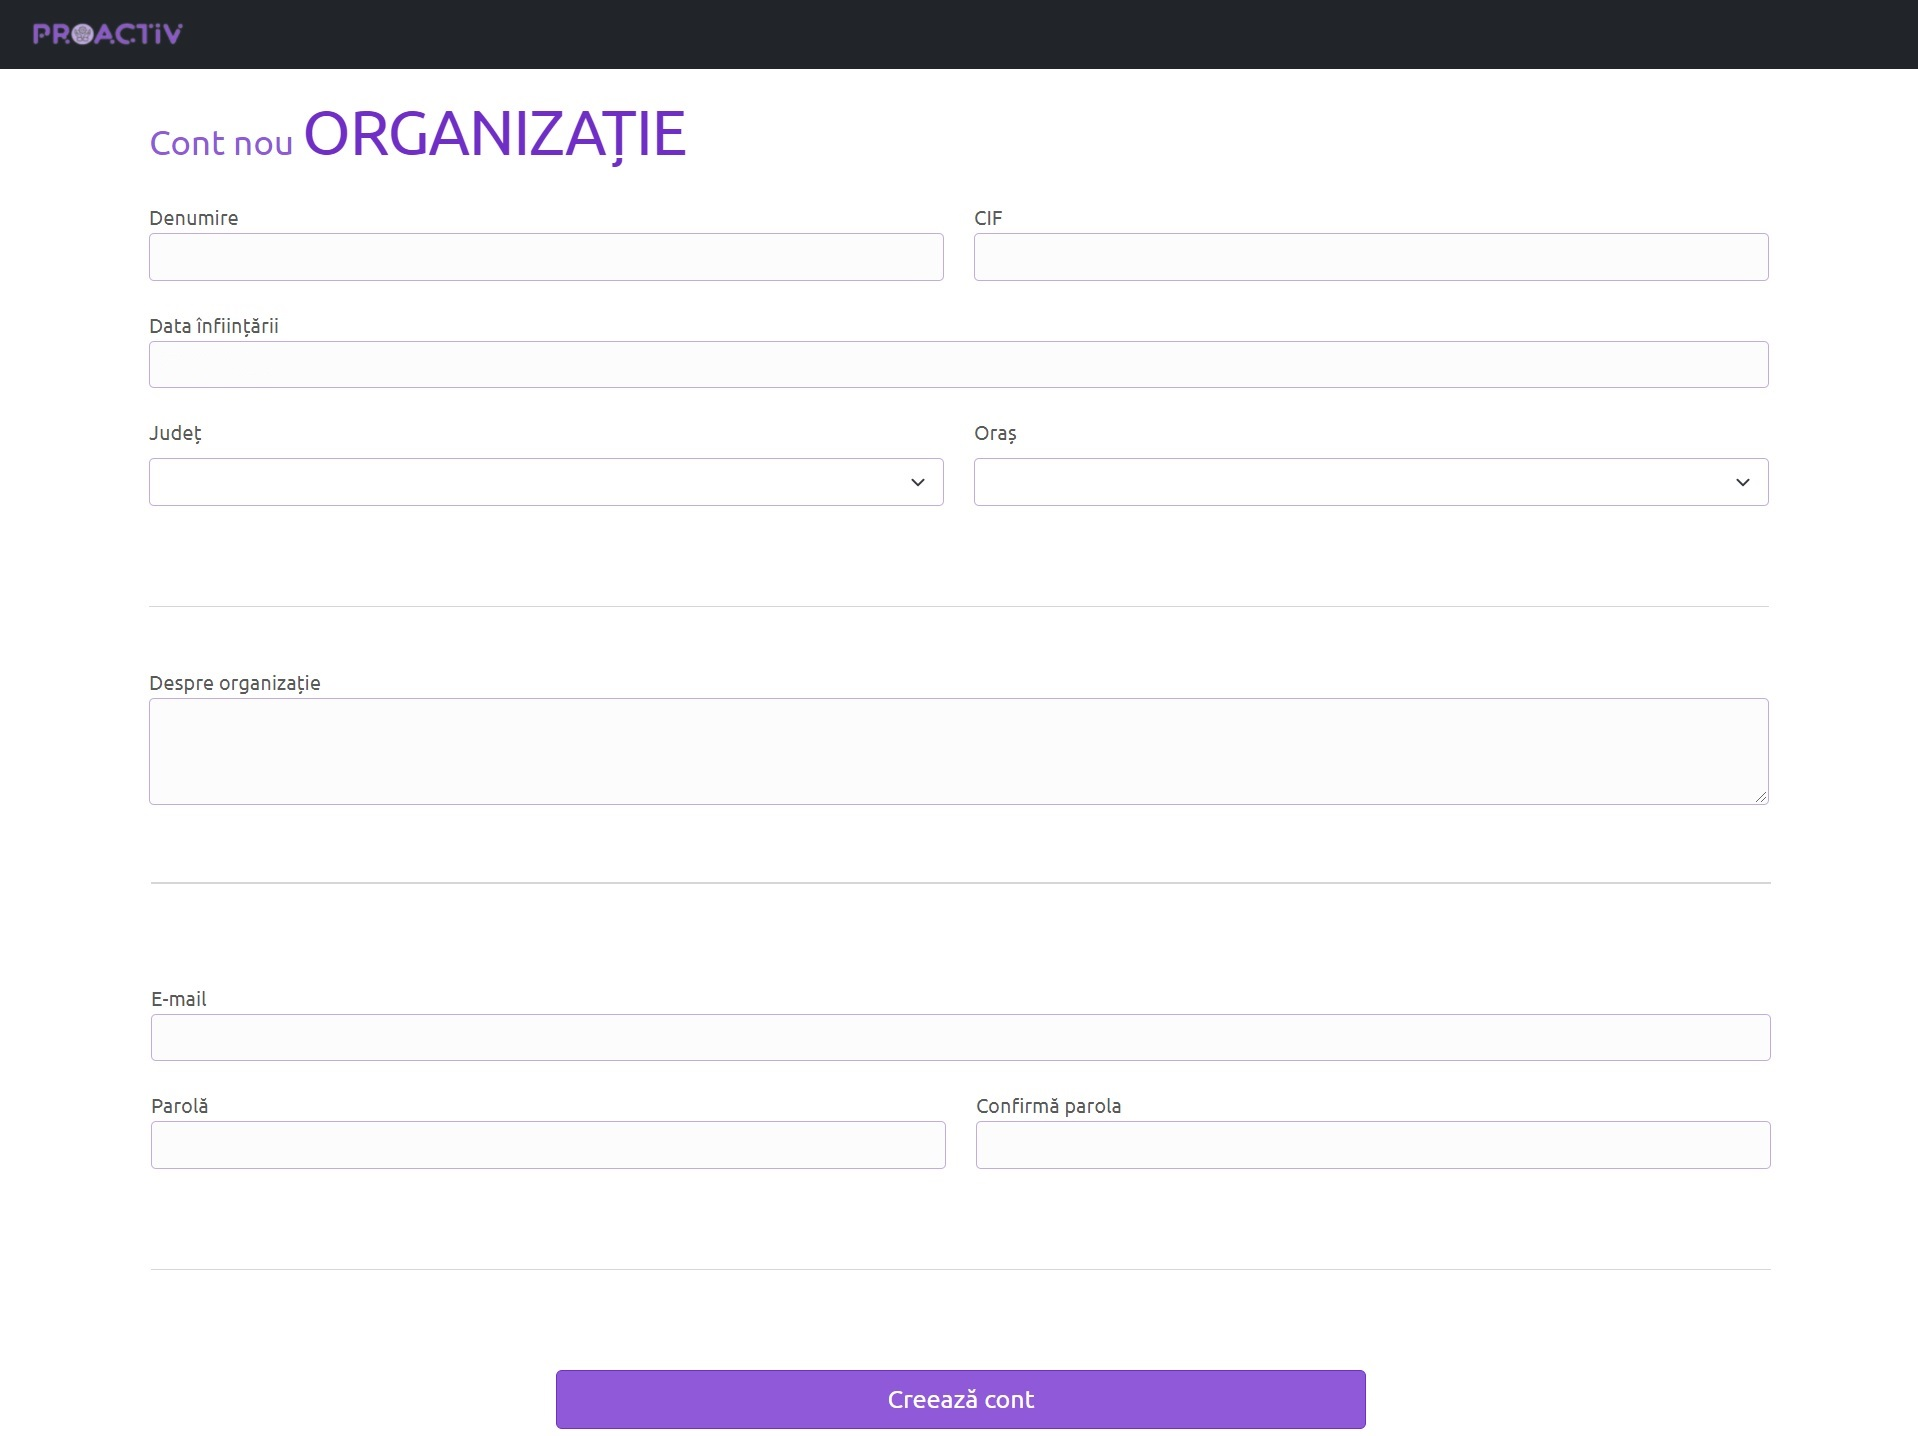
\includegraphics[width=1\linewidth]{./imagini/contorg.jpg}
  \caption{Pagina de înregistrare organizație a platformei Proactiv}
\end{figure}

\section{Contul meu}
\par
În momentul în care utilizatorul se autentifică, acesta este redirecționat către gestionarea propriului cont, indiferent dacă este voluntar sau reprezintă o organizație. Pagina “Contul meu” cuprinde un meniu de butoane care oferă diferite funcționalități. 
\\\par
La secțiunea “General”, utilizatorul își poate vedea datele personale în momentul înregistrării pe platformă și le poate modifica și actualiza, apăsând butonul “Actualizează”. Pagina va fi reîmprospătată, iar serverul îi va afișa un mesaj utilizatorului după actualizarea datelor lui, precum în Figura 2.10.
\\
\begin{figure}[H]
\centering
  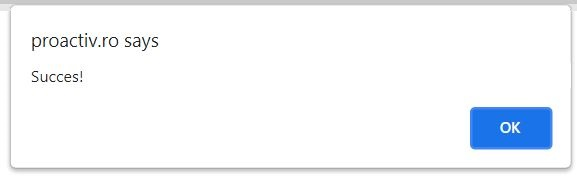
\includegraphics[width=0.5\linewidth]{./imagini/succes.jpg}
  \caption{Mesaj afișat după actualizarea datelor}
\end{figure}
\par
Desigur, datele și căsuțele de input diferă în funcție de tipul contului. Voluntarul își va putea modifica numele, prenumele și data nașterii, reprezentantul organizației va putea actualiza denumirea organizației, CIF-ul, data înființării și detaliile despre aceasta, iar ambele tipuri de cont vor putea modifica județul și orașul de reședință.
\\\par
Diferența dintre modurile de afișare a acestei secțiuni se poate observa făcând o comparație între Figurile 2.11 si 2.12.
\\
\begin{figure}[H]
\centering
  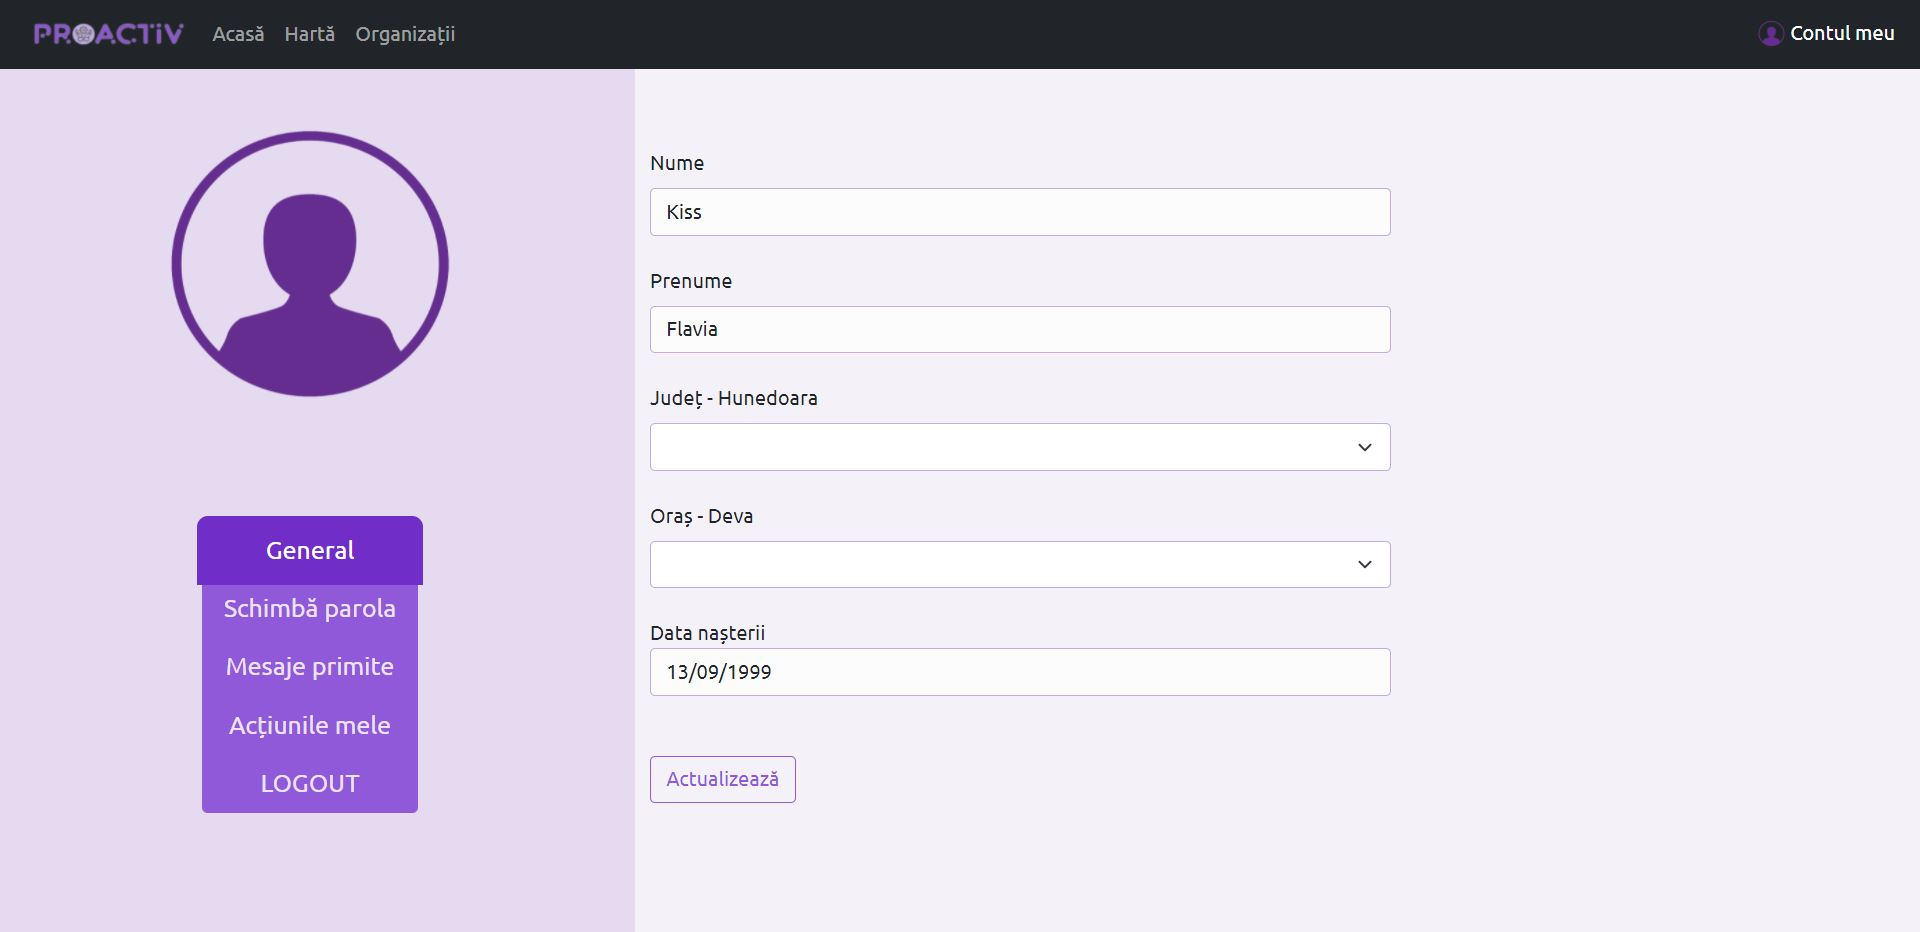
\includegraphics[width=1\linewidth]{./imagini/cont1.jpg}
  \caption{Pagina gestionare cont voluntar a platformei Proactiv}
\end{figure}
\begin{figure}[H]
\centering
  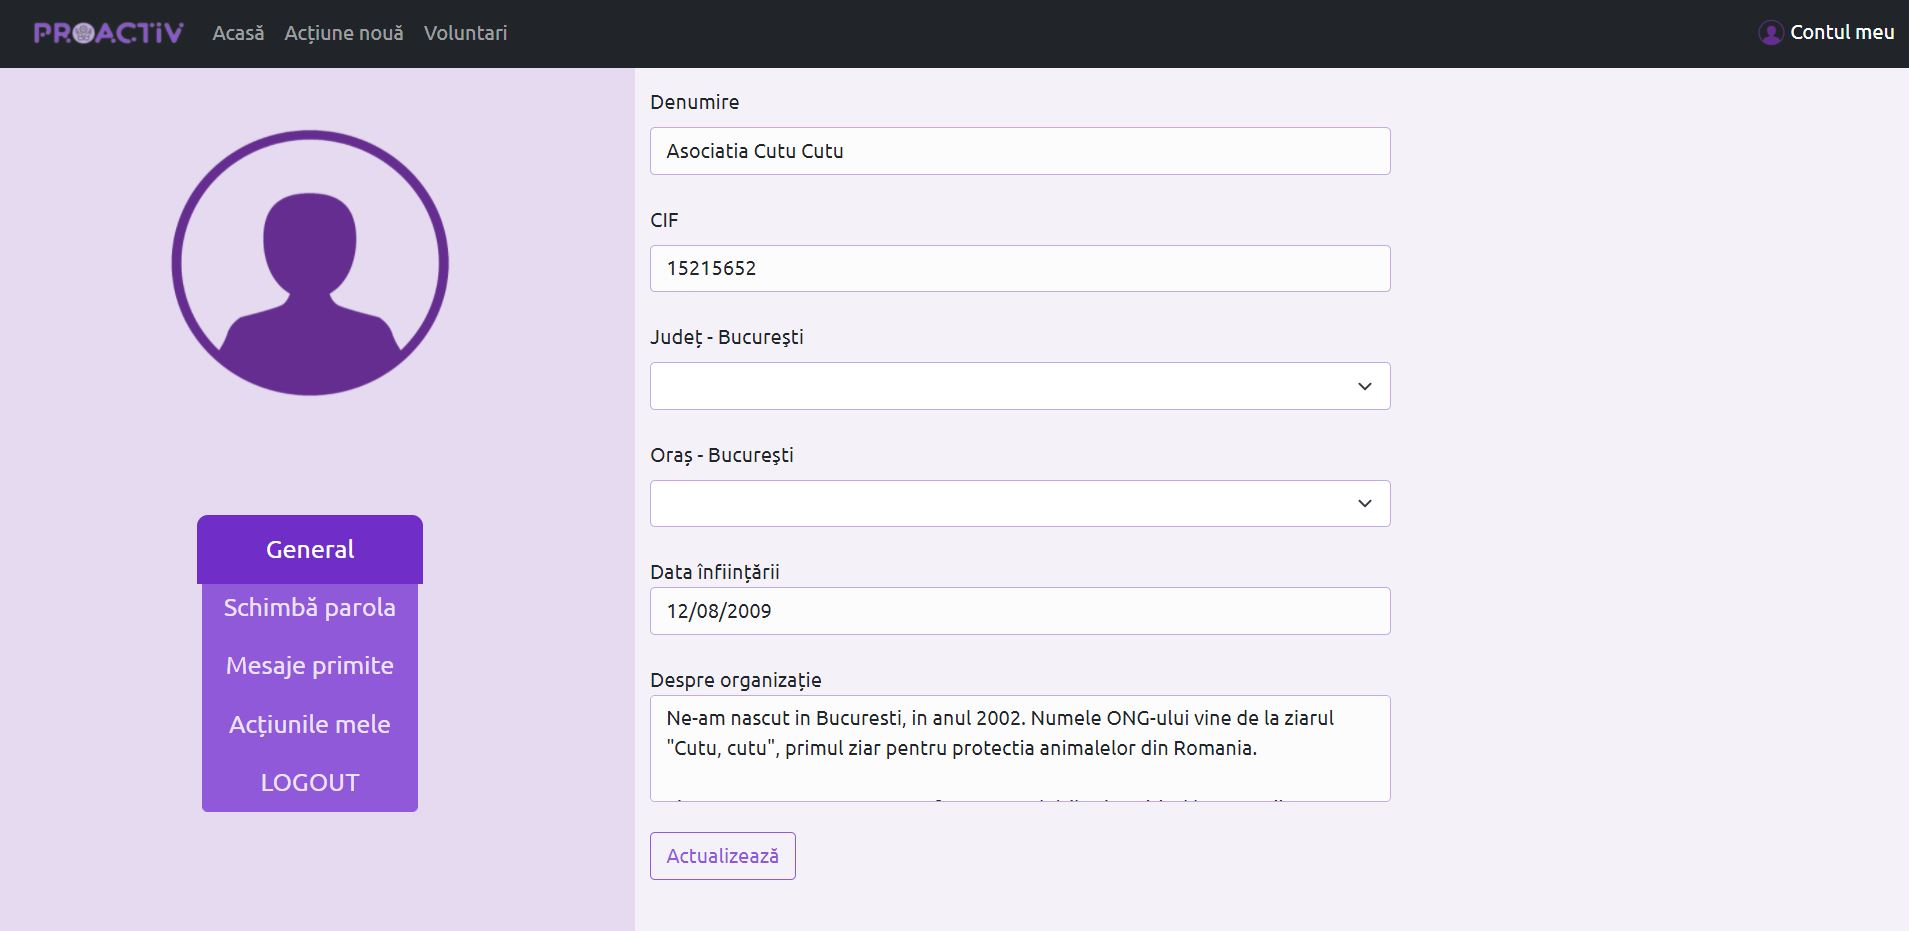
\includegraphics[width=1\linewidth]{./imagini/cont1org.jpg}
  \caption{Pagina gestionare cont organizație a platformei Proactiv}
\end{figure}
\par
La secțiunea “Schimbă parola”, ilustrată în Figura 2.13, utilizatorul își poate modifica parola, apăsând butonul cu același nume. Pentru ca actualizarea să se realizeze cu succes, acesta trebuie să introducă emailul și parola actuală corecte, iar parola nouă și confirmarea acesteia trebuie să corespundă și să fie diferite de parola veche.
\\
\begin{figure}[H]
\centering
  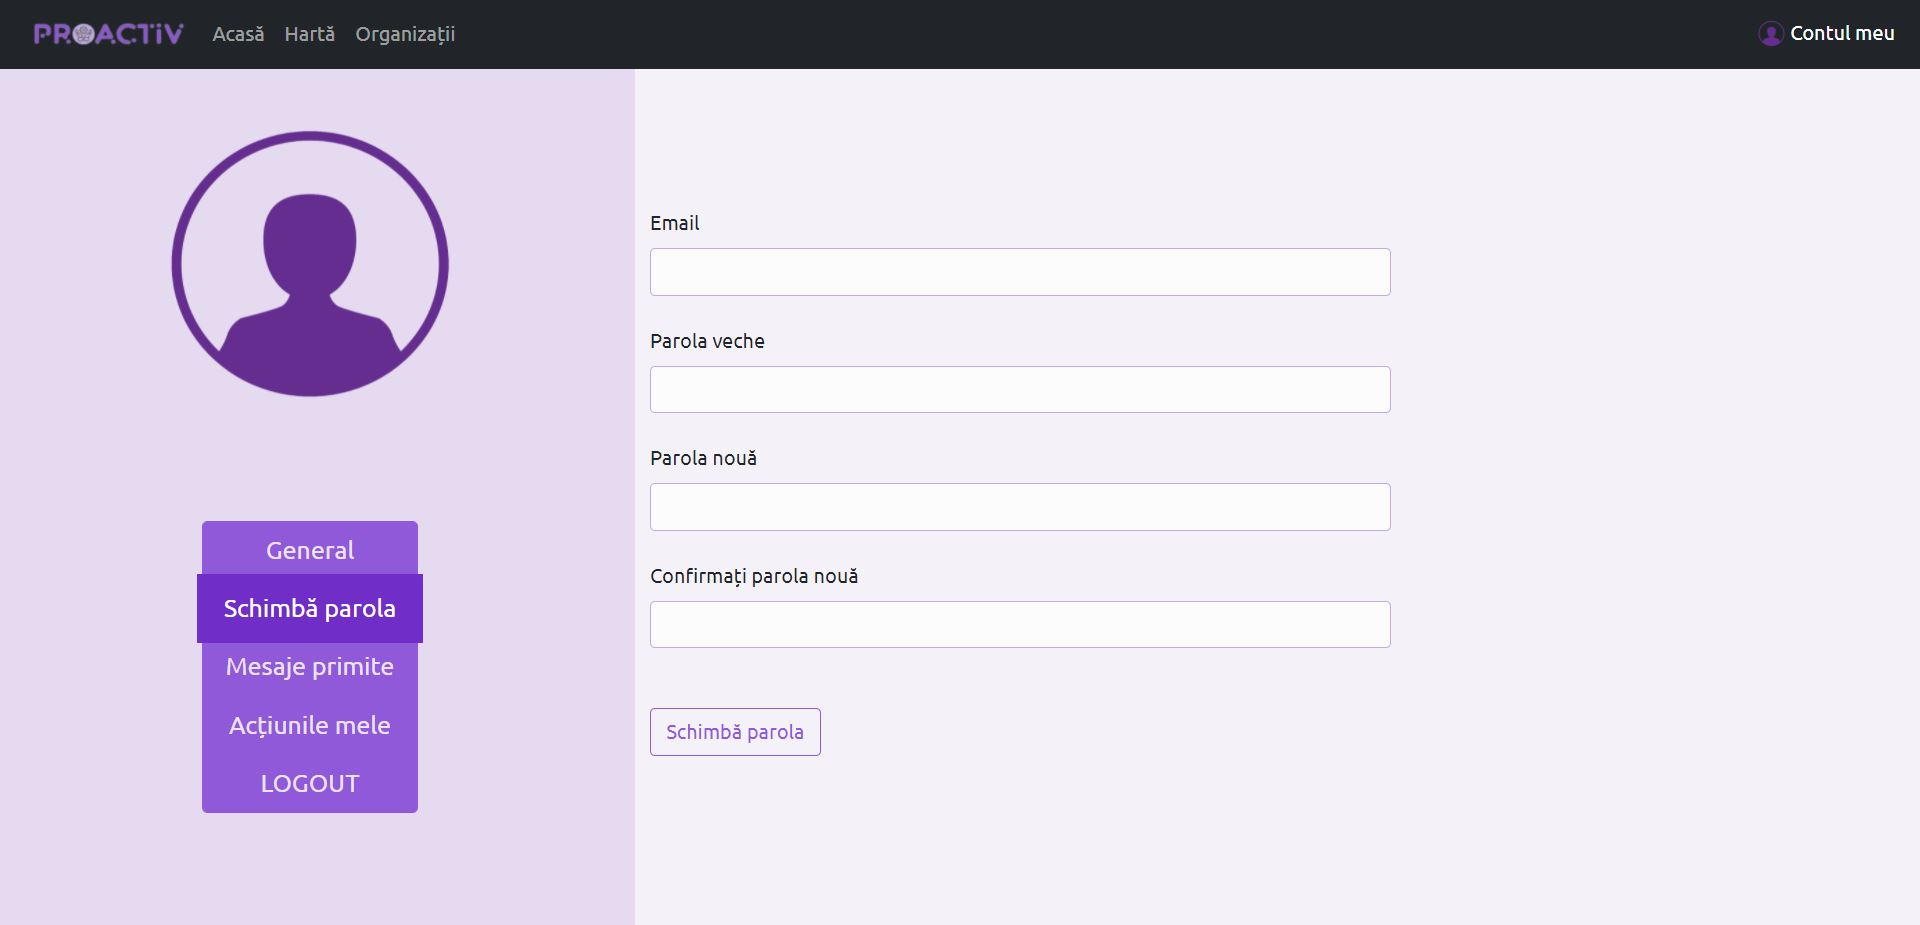
\includegraphics[width=1\linewidth]{./imagini/cont2.jpg}
  \caption{Secțiunea “Schimbă parola” a platformei Proactiv}
\end{figure}
\newpage
La secțiunea “Mesaje primite” sunt afișate mesajele primite de către utilizator, sub forma unor carduri Bootstrap. Acestea conțin denumirea organizației care a trimis mesajul, titlul și conținutul acestuia.
\par
La fel sunt prezentate și mesajele primite de către utilizatorii cu cont de tip organizație, dar în locul denumirii sunt afișate numele și prenumele voluntarului care a trimis mesajul.
\\
\begin{figure}[H]
\centering
  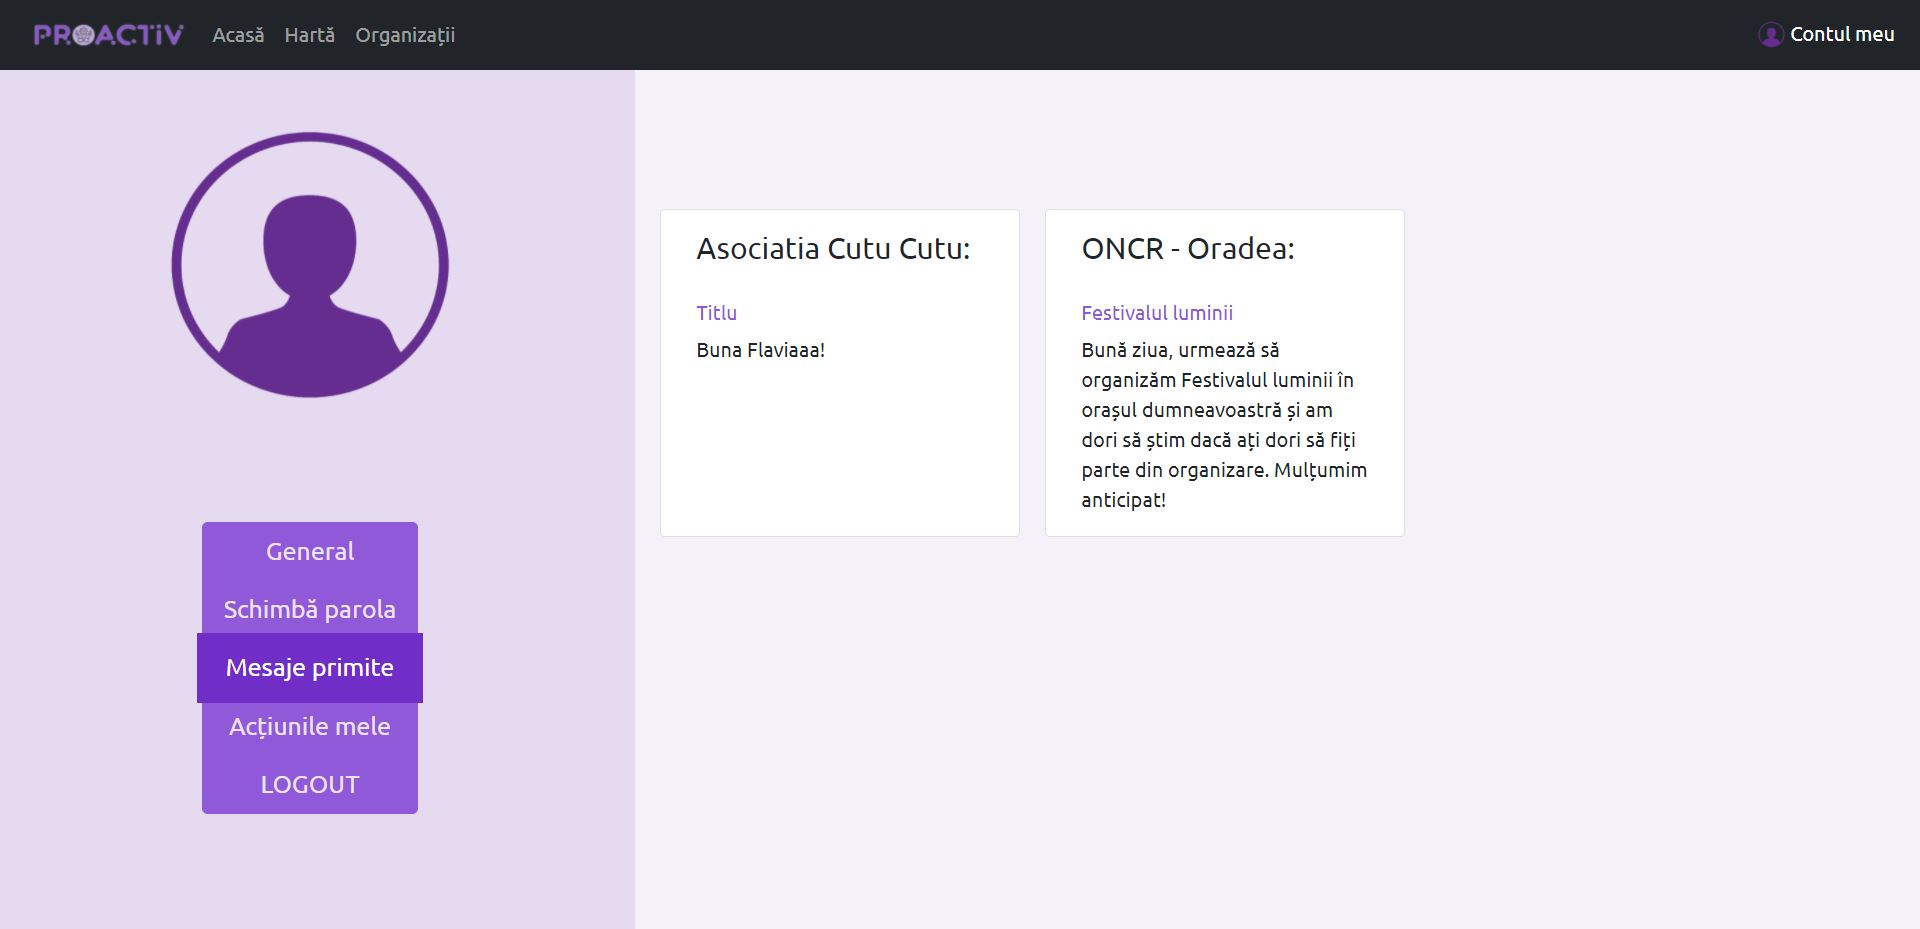
\includegraphics[width=1\linewidth]{./imagini/cont3.jpg}
  \caption{Secțiunea “Mesaje primite” a platformei Proactiv}
\end{figure}
\par
Iar la secțiunea “Acțiunile mele” sunt listate acțiunile semnalate de către utilizator, în cazul contului de tip organizație și acțiunile la care utilizatorul este înscris, în cazul voluntarilor.
\\
\begin{figure}[H]
\centering
  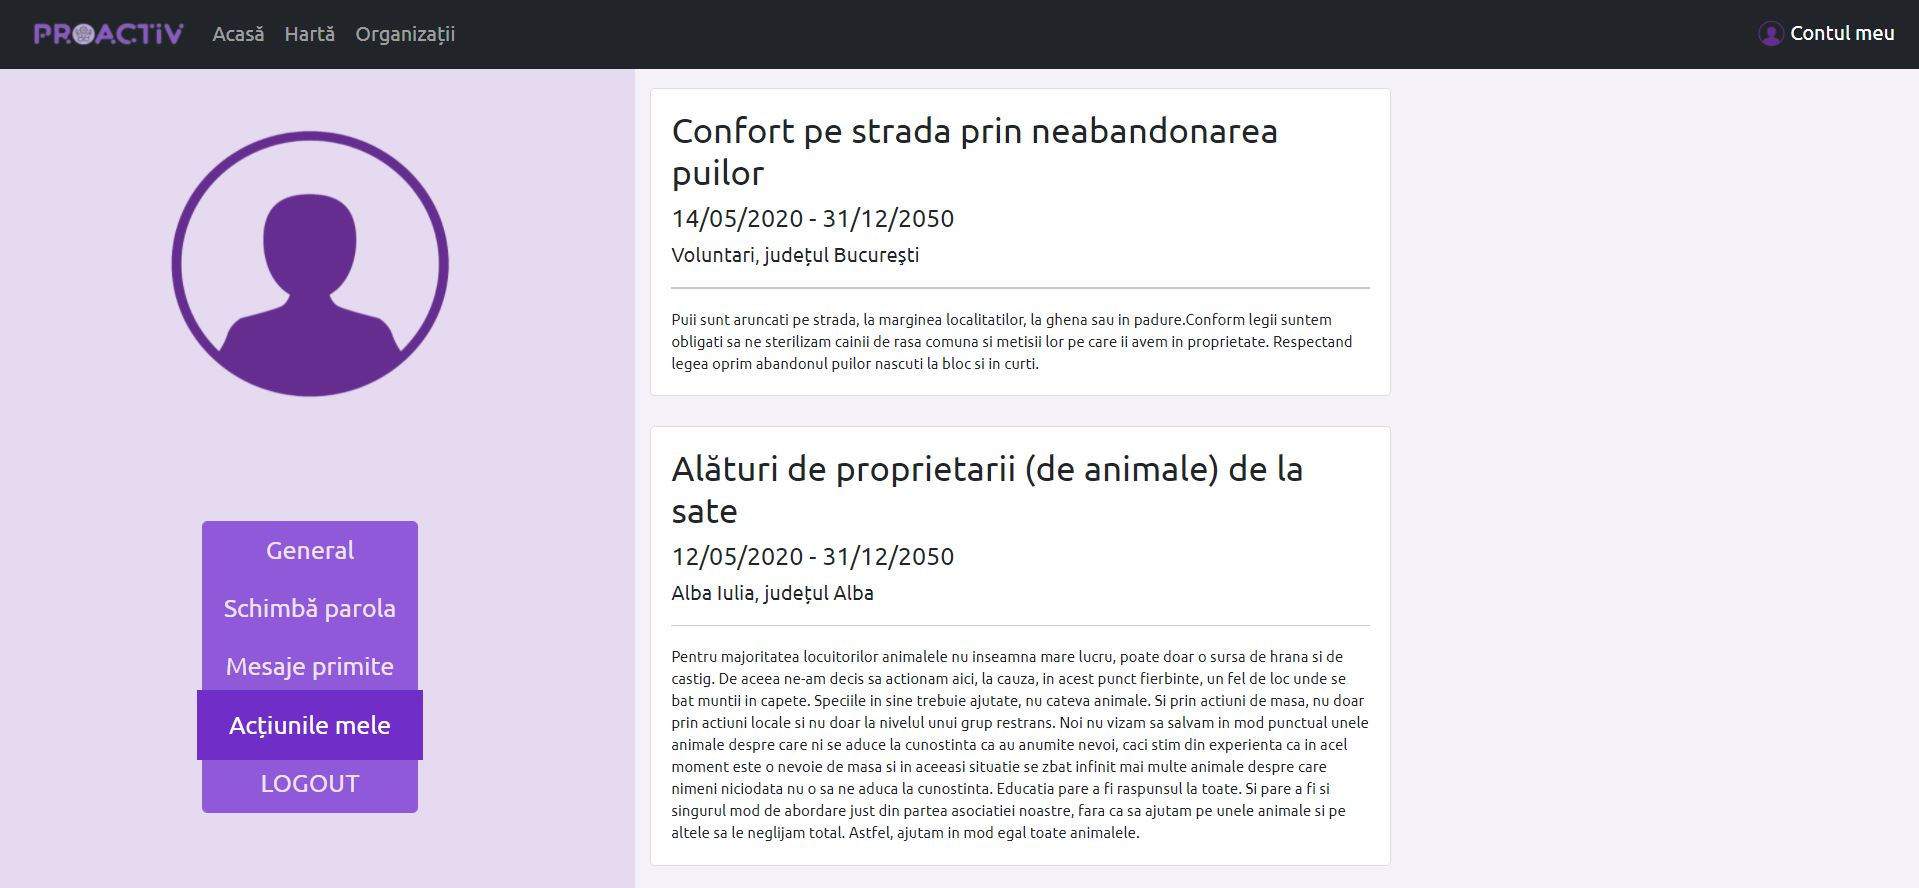
\includegraphics[width=1\linewidth]{./imagini/cont4.jpg}
  \caption{Secțiunea “Acțiunile mele” a platformei Proactiv}
\end{figure}

\section{Hartă}
\par
Pagina “Hartă” este vizibilă și accesibilă doar de către utilizatorii cu cont de tip voluntar. Aceasta cuprinde harta oferită de Google Maps API, centrată pe teritoriul României, cu diferiți pini afișați în funcție de acțiunile de voluntariat semnalate la momentul accesării paginii, de categoria în care sunt încadrate și de locația în care au loc acestea.
\\\par
În partea stângă a paginii se află o gamă de filtre, în cazul în care voluntarul dorește să vadă doar acțiunile semnalate într-un anumit județ, oraș sau doar dintr-o anumită categorie.
\\
\begin{figure}[H]
\centering
  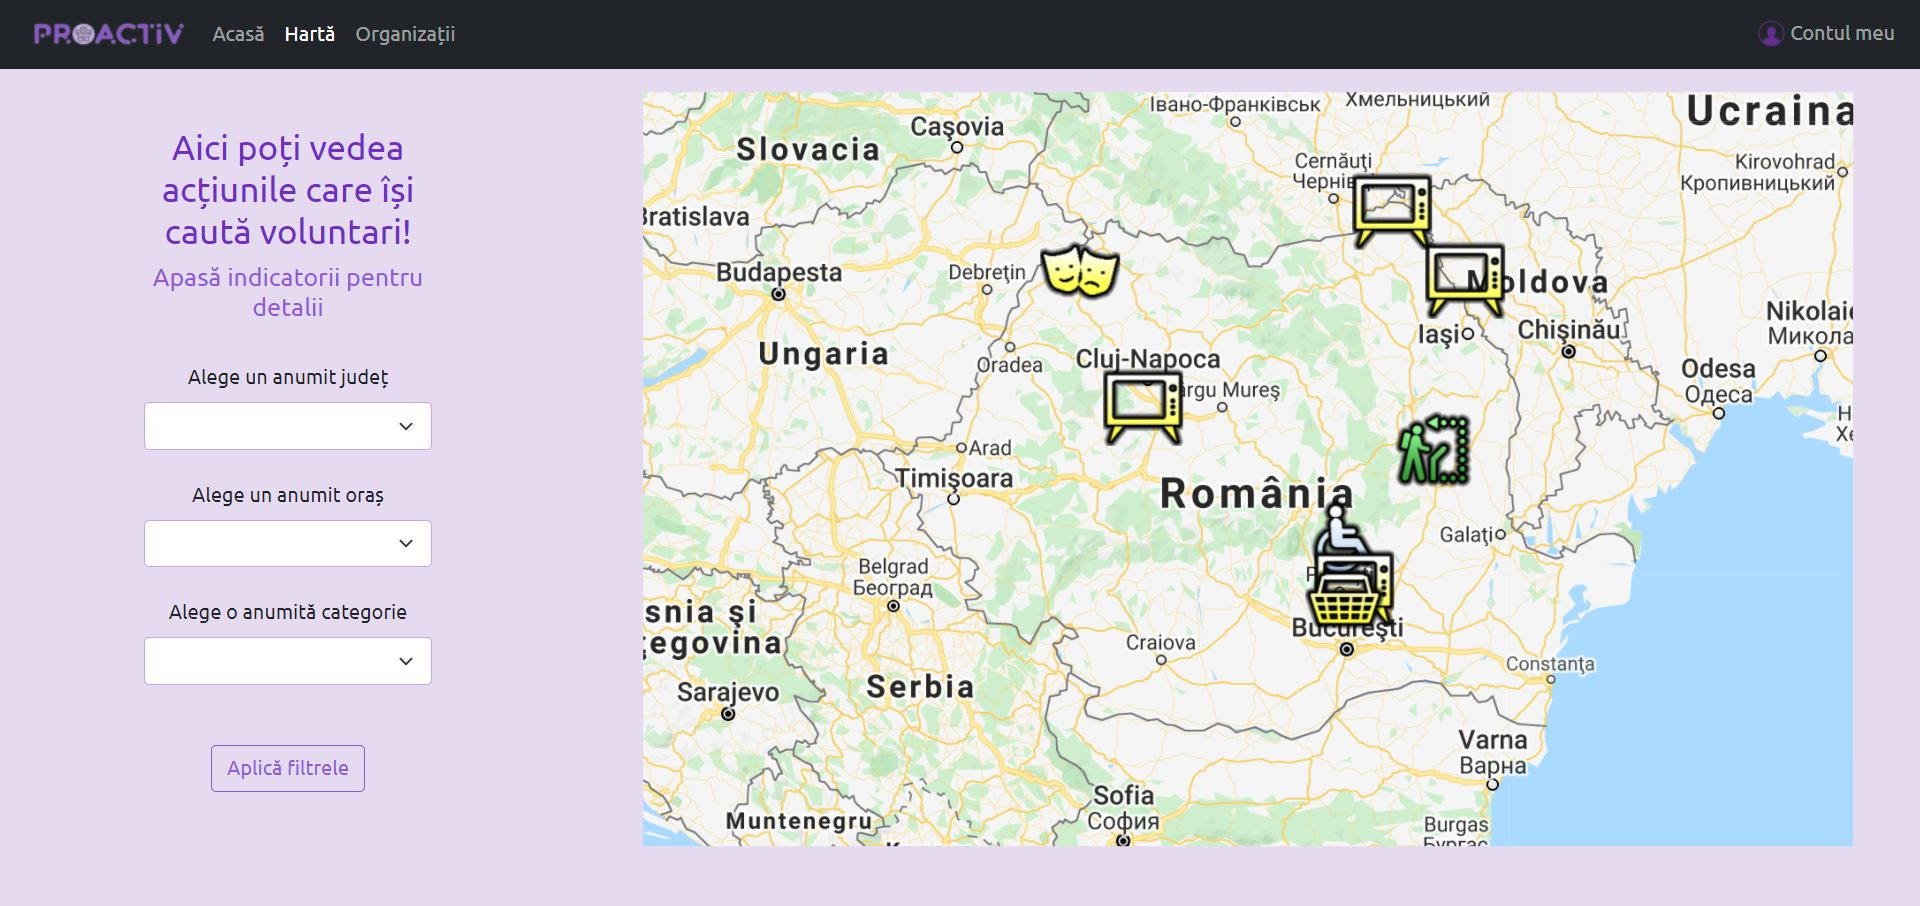
\includegraphics[width=1\linewidth]{./imagini/harta.jpg}
  \caption{Pagina “Hartă” a platformei Proactiv}
\end{figure}

\par
În momentul în care este apăsat un pin, se va deschide un pop-up cu detalii despre acesta, precum titlul, categoria în care se încadrează și perioada de desfășurare a acțiunii.
\\
\begin{figure}[H]
\centering
  
\includegraphics[width=0.4\linewidth]{./imagini/pin.jpg}
  \caption{Detalii despre un anumit pin apăsat}
\end{figure}

\section{Acțiune nouă}
\par
Această pagină este accesibilă doar de către utilizatorii cu tip de cont organizație.
\\ \par
Aceștia pot semnala o acțiune nouă de voluntariat, care ulterior va fi afișată pe hartă pentru ca utilizatorii cu tip de cont voluntar să se poată alătura ei. Datele cerute pentru această funcționalitate cuprind numele acțiunii, categoria din care aceasta face parte, o scurtă descriere a acesteia, intervalul și locația în care se desfășoară acțiunea respectivă.
\\
\begin{figure}[H]
\centering
  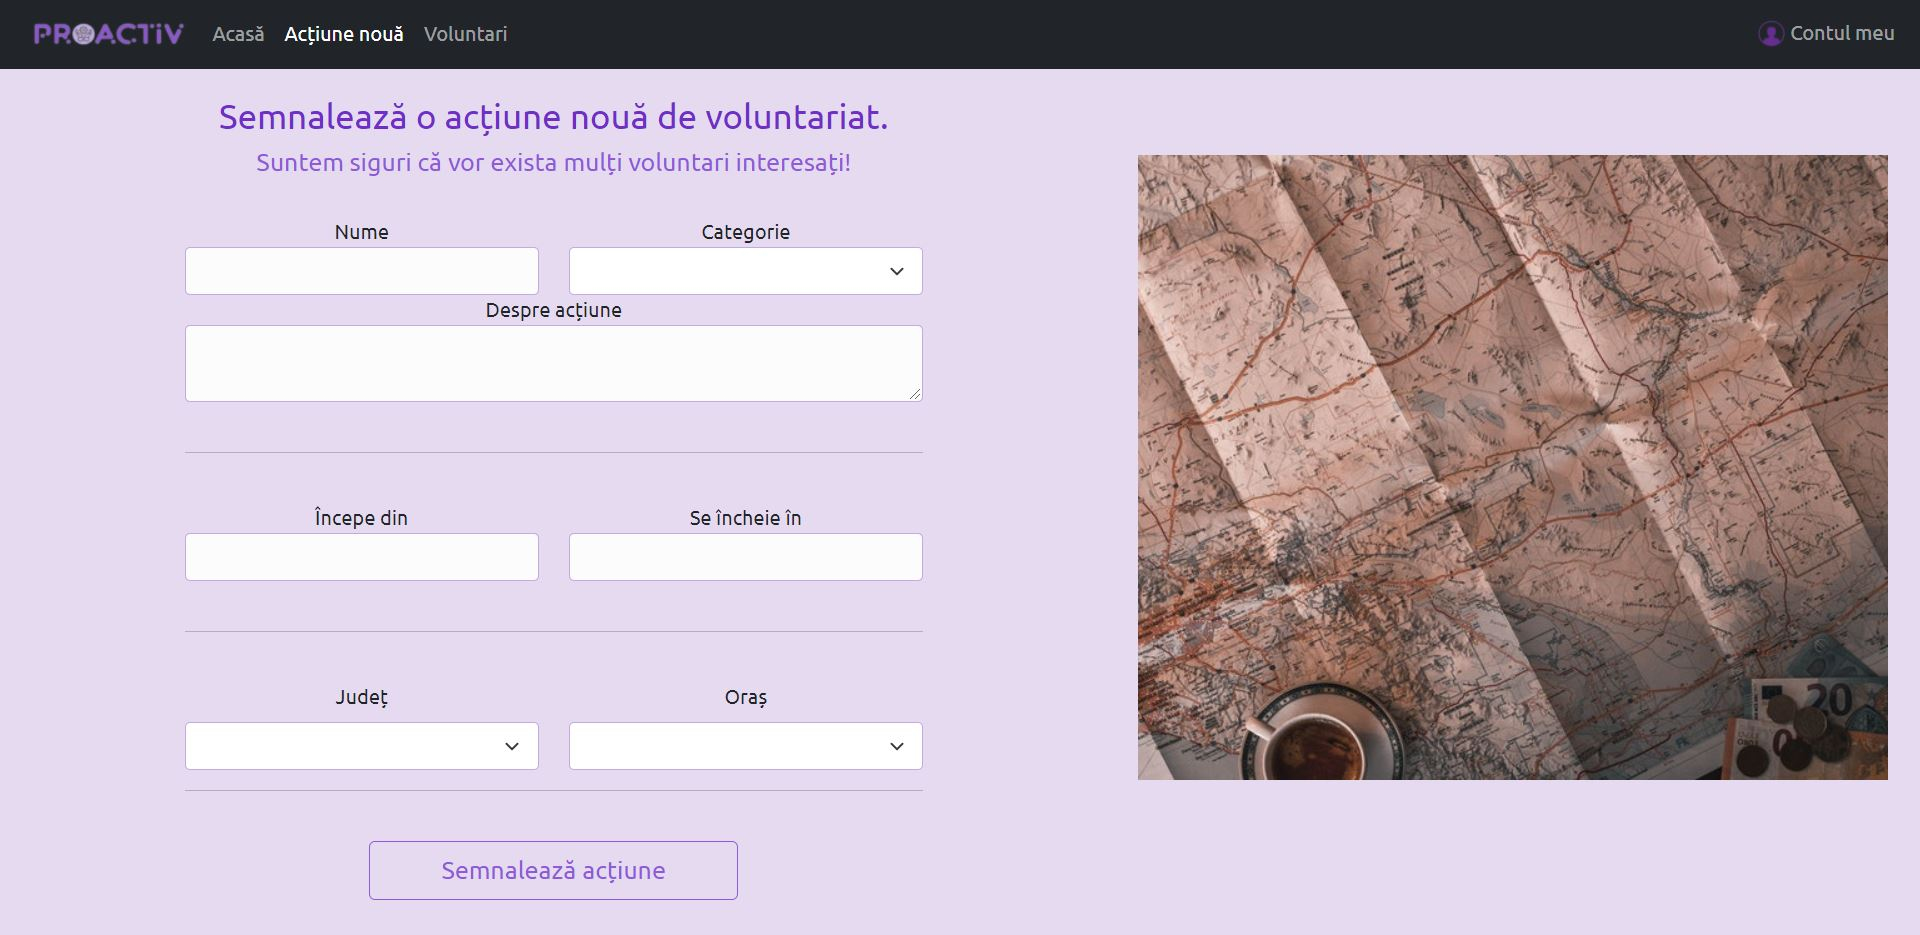
\includegraphics[width=1\linewidth]{./imagini/actiunenoua.jpg}
  \caption{Pagina “Acțiune nouă” a platformei Proactiv}
\end{figure}
\par
În momentul în care utilizatorul submite formularul, apăsând butonul “Semnalează acțiune”, pagina va fi reîmprospătată, iar serverul îi va afișa acestuia un răspuns pozitiv, pentru a-l anunța că operația a avut loc cu succes. 

\section{Voluntari}
\par
Pagina “Voluntari” a fost concepută pentru ca utilizatorii cu tip de cont organizație să poată lua legătura cu voluntarii înscriși pe platformă.
\\ \par
Pagina afișează în ordine alfabetică toți utilizatorii cu tip de cont voluntar, grupându-i pe trei coloane în funcție de numele acestora de familie, precum este ilustrat în Figura 2.19.
\begin{figure}[H]
\centering
  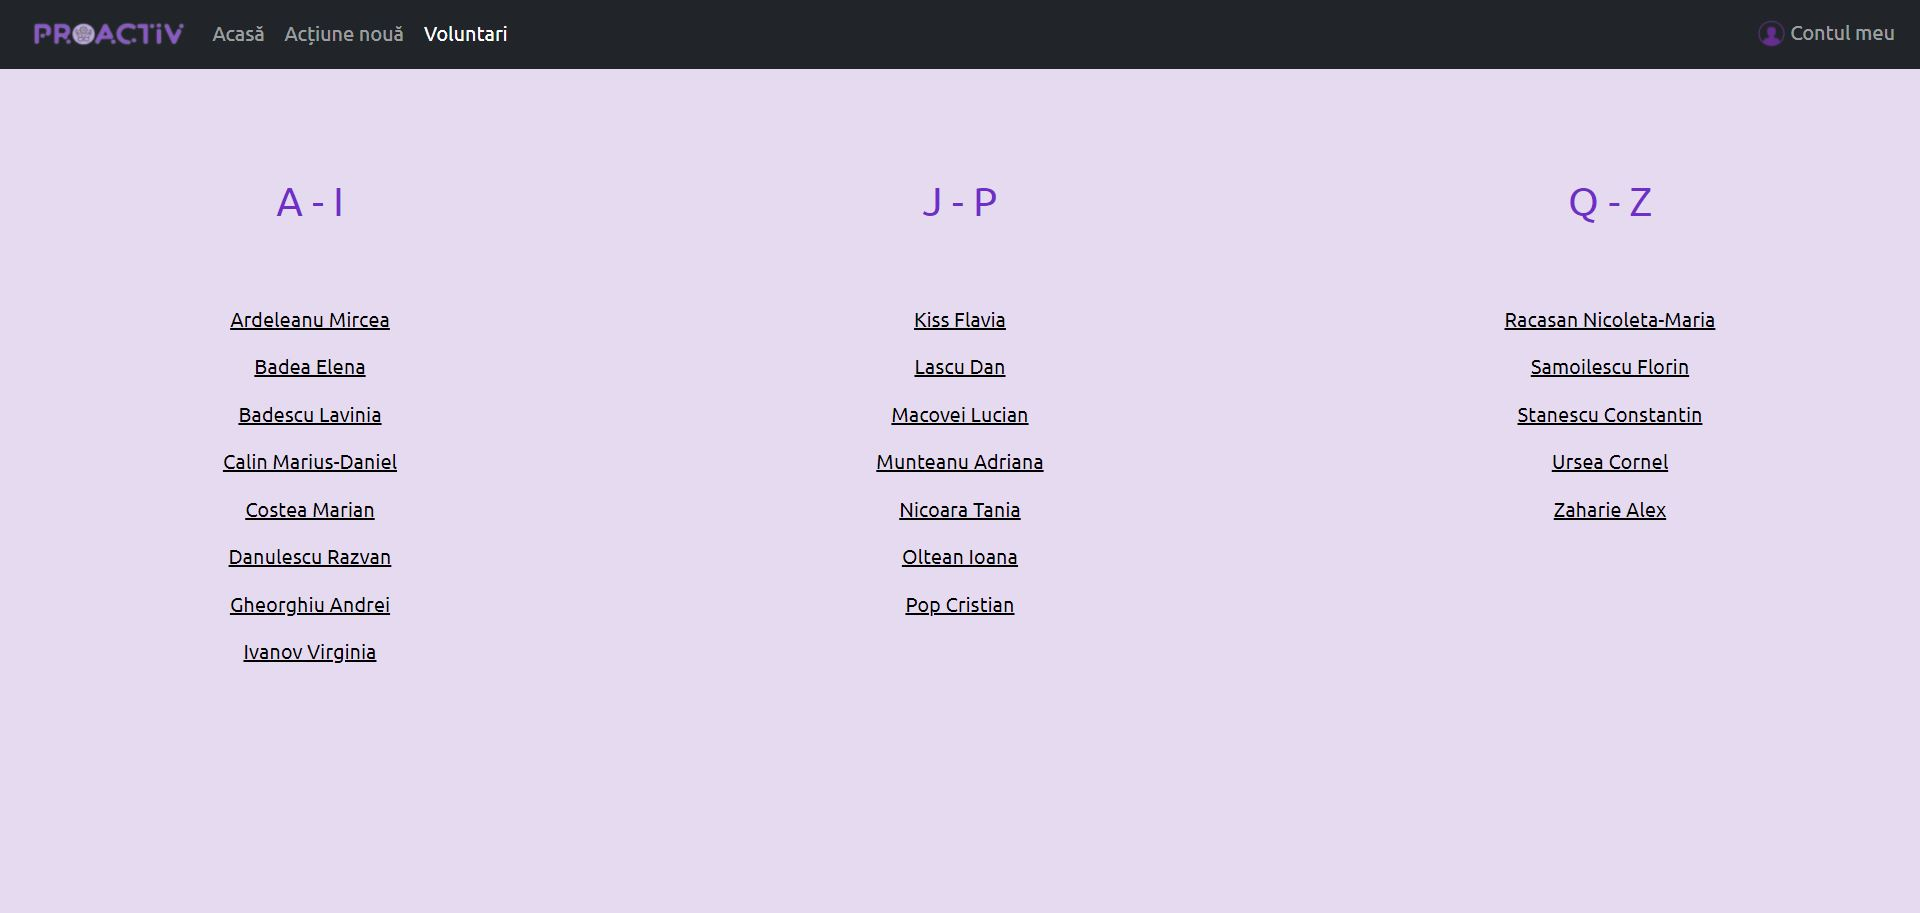
\includegraphics[width=0.95\linewidth]{./imagini/vol1.jpg}
  \caption{Pagina “Voluntari” a platformei Proactiv}
\end{figure}
\par
Atunci când este apăsat un anumit voluntar, se deschide o fereastră modal unde sunt afișate atât detalii despre voluntarul respectiv, cât și o secțiune pentru a trimite un mesaj. Pentru a face acest lucru, este obligatorie completarea căsuțelor text care reprezintă titlul și conținutul mesajului care se dorește a fi trimis.
\par
În cazul în care utilizatorul nu dorește să trimită un mesaj voluntarului, ci doar să vadă mai multe detalii despre acesta, poate părăsi fereastra apăsând butonul “X” din colțul dreapta-sus.
\begin{figure}[H]
\centering
  
\includegraphics[width=0.95\linewidth]{./imagini/vol2.jpg}
  \caption{Pagina “Voluntari” a platformei Proactiv}
\end{figure}

\section{Organizații}
\par
Pagina “Organizații” are același scop ca și pagina descrisă anterior, dar este accesibilă utlizatorilor cu tip de cont voluntar.
\\\par
În locul listei de voluntari, este afișată lista tuturor organizațiilor înscrise pe site la momentul accesării paginii, iar apăsarea unui element din listă va duce la afișarea detaliilor importante despre organizația respectivă și la posibilitatea voluntarului de a trimite un mesaj acesteia.
\\
\begin{figure}[H]
\centering
  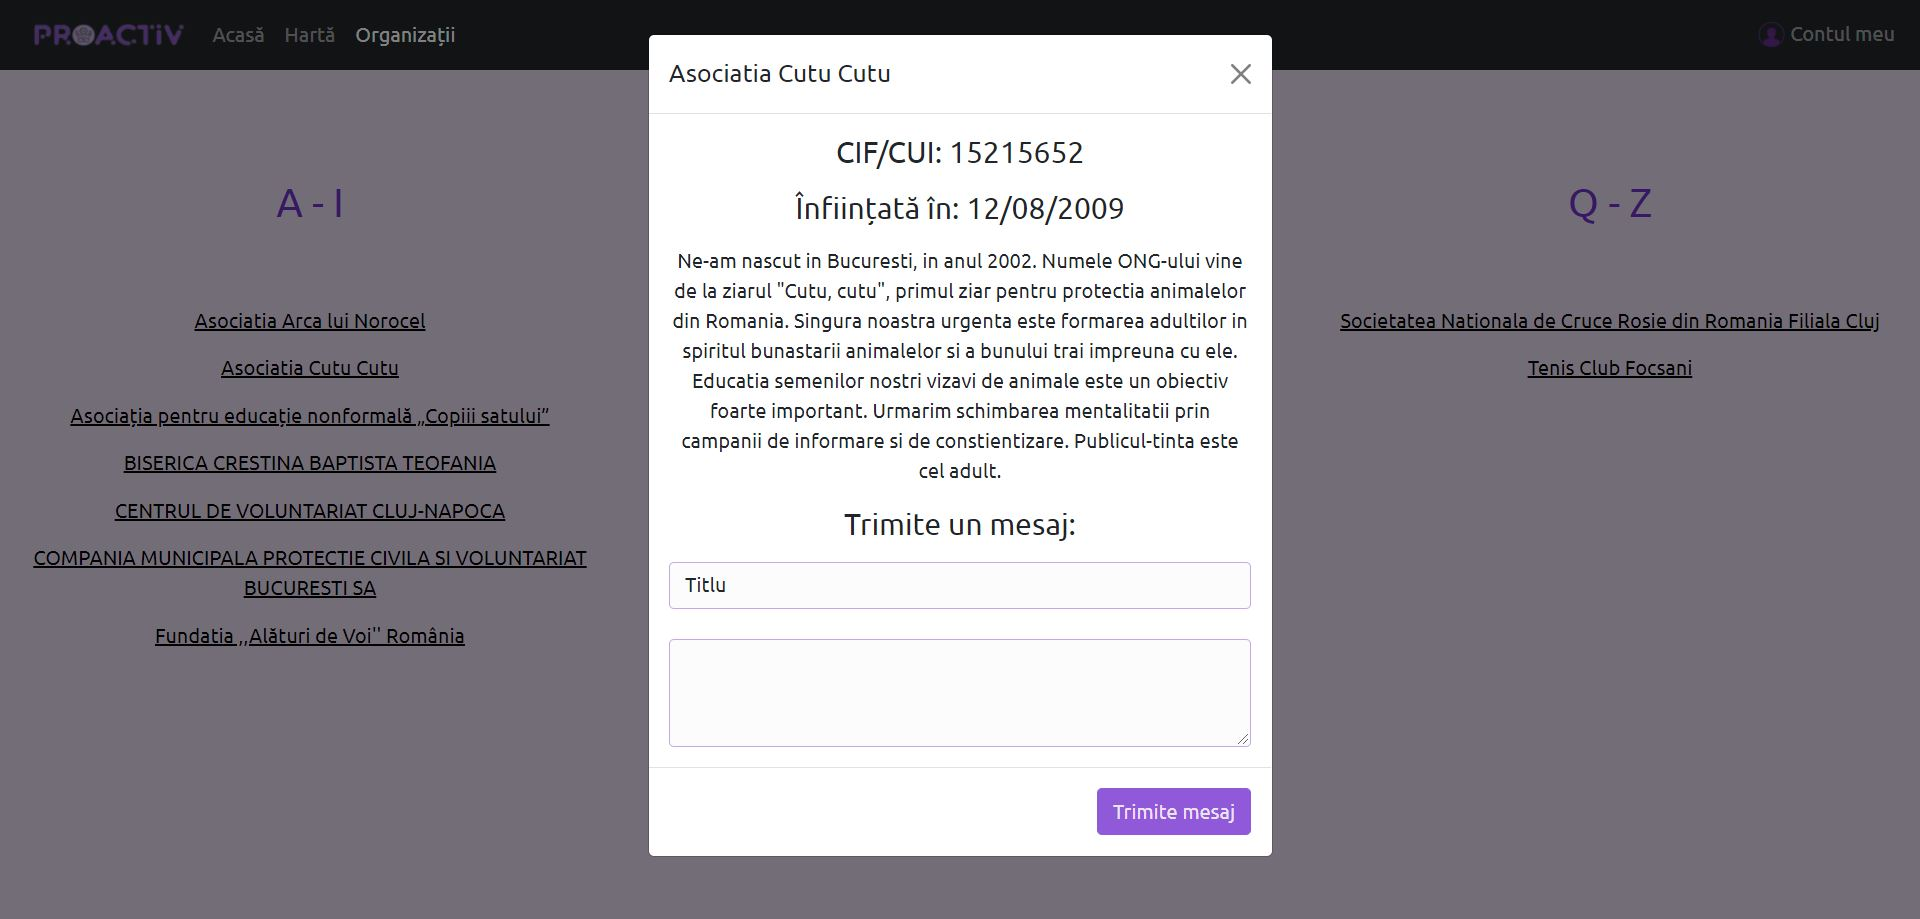
\includegraphics[width=1\linewidth]{./imagini/org.jpg}
  \caption{Pagina “Organizații” a platformei Proactiv}
\end{figure}

\chapter{Funcționalitatea aplicației}
\section{Modelarea funcționalității}
\par
Diagrama cazurilor de utilizare oferă o descriere generală a modului în care va fi utilizat sistemul și surprinde modul în care sistemul interacționează cu unul sau mai mulți actori \cite{usecases}.
\\
\par
Figura 3.1 ilustrează diagrama de cazuri a aplicației Proactiv. Actorii includ voluntarul și organizația, iar sistemul este subiectul cazurilor de utilizare, clasa a cărui comportament îl descriu aceste cazuri. 
În momentul în care utilizatorul intră pe site, acesta are posibilitatea de a parcurge pagina principală, de a se autentifica sau de a se înregistra. Excluzând aceste trei cazuri menționate anterior, restul cazurilor sunt condiționate de autentificarea utilizatorului pe platformă.
\\
\begin{figure}[h!]
  \centering
    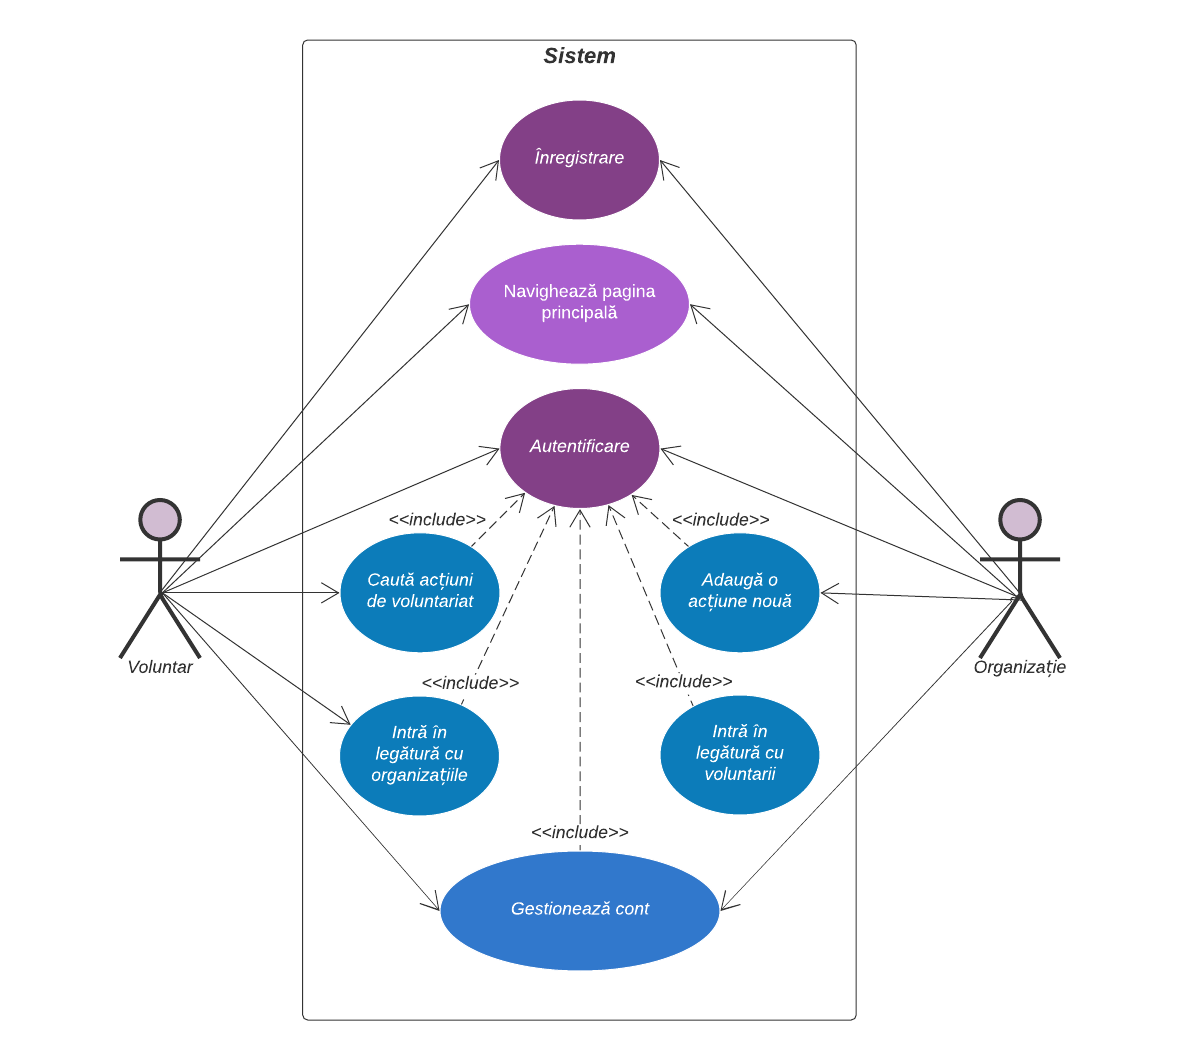
\includegraphics[width=0.7\linewidth]{./imagini/UseCase.png}
    \caption{Diagrama de cazuri a aplicației Proactiv}
\end{figure}

\par
Diagrama de secvențe la nivel de sistem are rolul de a modela interacțiunile dintre actorii externi și sistem.
\\
\par
În cazul aplicației Proactiv, interacțiunea dintre sistem și actorul Utilizator este una simplă. După ce actorul introduce credențialele necesare autentificării, sistemul verifică corectitudinea acestora și oferă utilizatorului acces pe platformă. Sistemul actualizează datele și le afișează utilizatorului.
\\
\begin{figure}[h]
\centering
  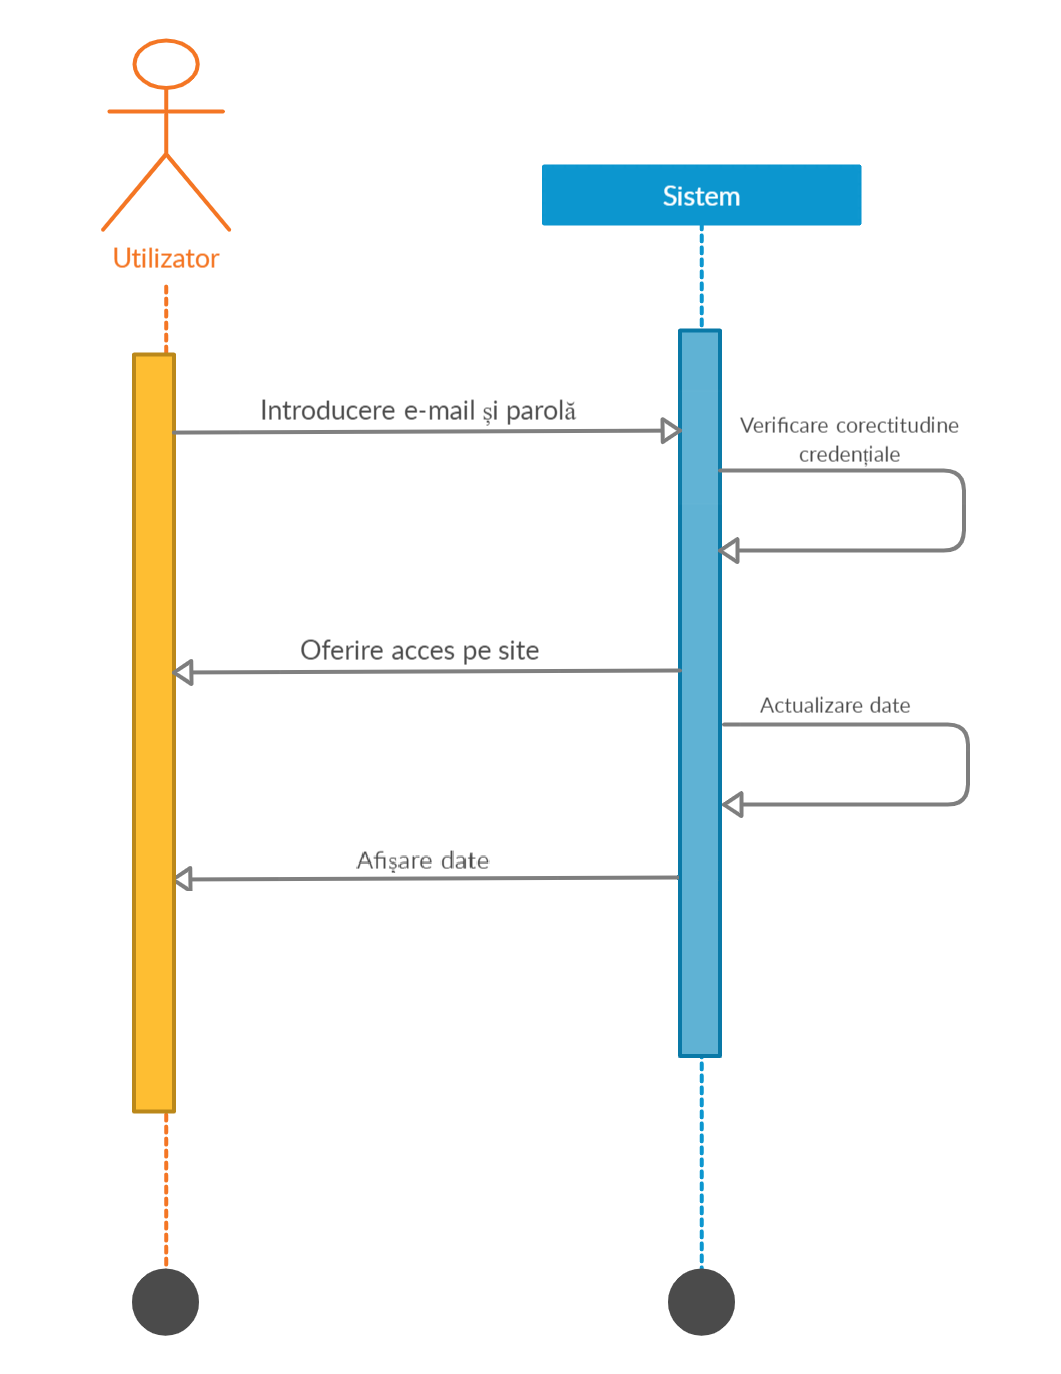
\includegraphics[width=0.6\linewidth]{./imagini/Sequence.jpg}
  \caption{Diagrama de secvente a aplicației Proactiv}
\end{figure}


\newpage

\section{Modelarea comportamentului aplicației în context}
\par
Diagrama de activitate ilustrează modul în care sunt procesate datele pe măsură ce parcurg sistemul. Urmărirea şi documentarea asocierii datelor cu un proces este utilă în dezvoltarea înţelegerii sistemului în ansamblu \cite{uml}.
\\
\par
În Figura 3.3 este descrisă activitatea platformei pornind de la verificarea existenței unui cont al utilizatorului. Daca acesta este inexistent, intervine etapa de înregistrare, urmată de autentificare și de oferirea accesului pe site. Sistemul verifică tipul de cont și afișează informațiile aferente acestuia.
\\
\begin{figure}[h!]
\centering
  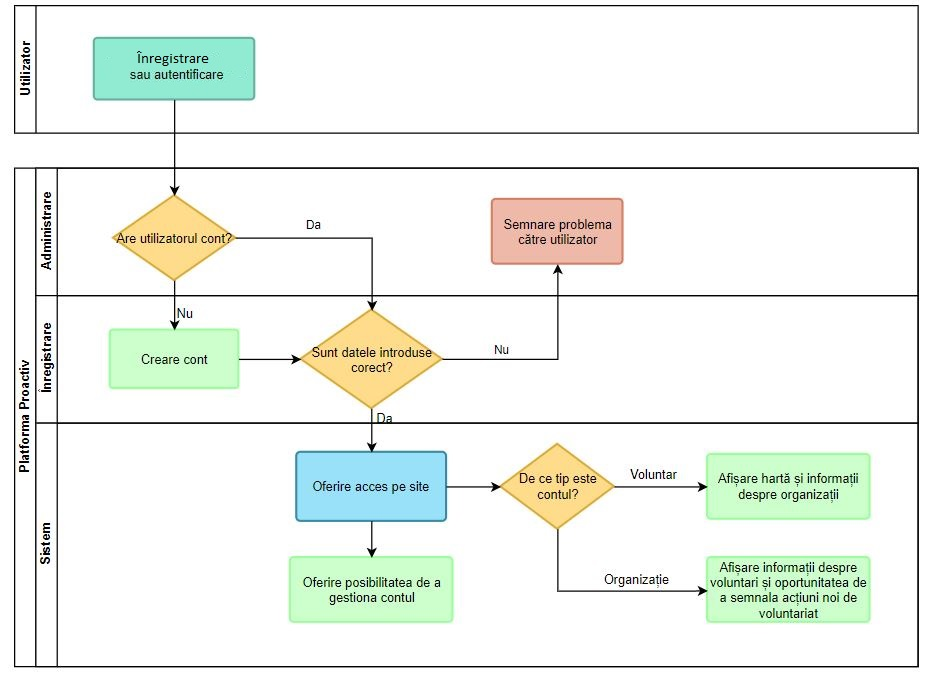
\includegraphics[width=1\linewidth]{./imagini/swimlane.JPG}
  \caption{Diagrama de activitate a aplicației Proactiv}
\end{figure}

\newpage
\par
Diagrama de stări şi tranziţii la nivel de sistem descrie toate stările pe care un obiect le poate avea, evenimentele datorită cărora un obiect tranzitează dintr-o stare în alta, condițiile care trebuie îndeplinite înainte ca tranziția să aibă loc și acțiunile întreprinse în timpul vieții obiectului.
\par
Aceste diagrame sunt foarte utile pentru descrierea comportamentului obiectelor individuale în cadrul întregului set de cazuri de utilizare care afectează acele obiecte.

\begin{figure}[h!]
\centering
  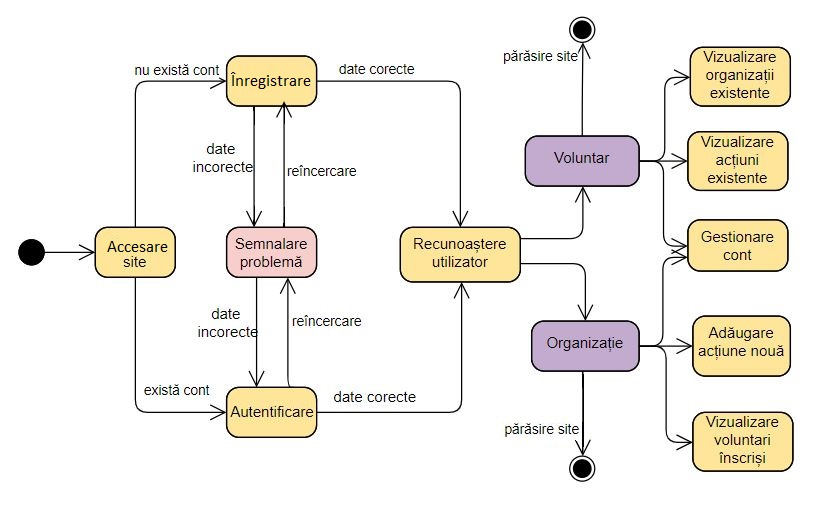
\includegraphics[width=0.9\linewidth]{./imagini/stateMachine.JPG}
  \caption{Diagrama de stări și tranziții a aplicației Proactiv}
\end{figure}

\newpage

\section{Înregistrarea}
\par
Înregistrarea pe platforma Proactiv se poate accesa din pagina principală, apăsând unul dintre butoanele  “VOLUNTAR” sau  “ORGANIZAȚIE”, în funcție de tipul de cont pe care utilizatorul dorește să îl dețină. După apăsarea unuia dintre butoane, utilizatorul este redirecționat fie către pagina de  “Cont nou Voluntar”, fie către cea de  “Cont nou Organizație”.
\\
\par
Aceste două pagini menționate anterior constau dintr-un formular care cuprinde diferite tipuri de căsuțe de input, în funcție de datele necesare creării unui cont de un anumit tip. Pentru a submite formularul apăsând butonul  “Creează cont”, utilizatorul este condiționat de completarea tuturor câmpurilor de input. 
\\
\par
După submiterea formularului, sistemul verifică dacă anumite criterii sunt îndeplinite, precum faptul că nu există deja un cont cu email-ul introdus și că parolele introduse corespund. Dacă răspunsul este unul pozitiv, datele sunt adăugate în baza de date și utilizatorul este redirecționat către pagina principala, unde se poate autentifica cu contul nou creat. Daca răspunsul este negativ, problema va fi semnalată acestuia, oferindu-i-se șansa să modifice datele și să reîncerce.
\\
\lstset{showstringspaces=false}
\begin{lstlisting}[basicstyle=\small, language=PHP]{Name=contvoluntar.php}
// Verificam emailul
$sql = "SELECT idVoluntar FROM voluntar WHERE email = \"".$email."\"";
$sql2 = "SELECT idOrganizatie FROM organizatie WHERE email = \"".$email."\"";
$result = mysqli_query($link, $sql);
$result2 = mysqli_query($link, $sql2);
$resultCheck = mysqli_num_rows($result);
$resultCheck2 = mysqli_num_rows($result2);
if ($resultCheck > 0 || $resultCheck2 > 0){
   $email_err = "Acest e-mail este deja utilizat";
}
// Verificam parola
if($password != $confirm_password){
   $confirm_password_err = "Parolele nu se potrivesc";
}
// Verificam lipsa erorilor inainte de a insera datele in baza de date
if(empty($email_err) && empty($confirm_password_err)){
   // Statement-ul de insert
   $sql = "INSERT INTO voluntar (idVoluntar,nume,prenume,dataN,".
          "judet,oras,email,parola) VALUES (?,?,?,?,?,?,?,?)";
   if($stmt = mysqli_prepare($link, $sql)){
      // Transformam parola in hash code
      $hashed_password = password_hash($password, PASSWORD_DEFAULT); 
      mysqli_stmt_bind_param($stmt, "dsssssss", $id, $nume, $prenume,
                          $datan, $judet, $oras, $email, $hashed_password);

      // Executam statement-ul
      if(mysqli_stmt_execute($stmt)){
         // Redirectionam catre pagina principala
         header("location: paginaPrincipala.php");
      } else{
         echo '<script>'.
         'alert("Oops! Ceva nu a mers bine! '.
         'Va rog sa reveniti mai tarziu");</script>';
      }
      // Inchidem statement-ul
      mysqli_stmt_close($stmt);
   }
}
\end{lstlisting}

\section{Autentificarea}
\par
Autentificarea pe platforma Proactiv se poate face din pagina principală, apăsând butonul  “Loghează-te” din prima secțiune a caruselului de imagini. După apăsarea butonului se va deschide un modal unde pot fi introduse credențialele, anume email și parolă.
\\
\par
După completarea acestor două câmpuri de imput, utilizatorul poate apăsa butonul din partea inferioară a modalului. În momentul submiterii credențialelor, sistemul preia datele introduse de utilizator, le caută în baza de date și în cazul unui răspuns pozitiv, pornește sesiunea, inițializează variabilele acesteia și redirecționează utilizatorul către contul lui, oferindu-i-se acces la funcționalitățile platformei aferente tipului de cont.
\\
\begin{lstlisting}[basicstyle=\small, language=PHP]{Name=paginaPrincipala.php}
//Preluam credentialele introduse de catre utilizator
$username = $_POST["username"];
$password = $_POST["password"];

// Validam credentialele
if(empty($username_err) && empty($password_err)){
   $sql1 = "SELECT idVoluntar FROM voluntar WHERE email = \"".$username."\"";
   $sql2 = "SELECT idOrganizatie FROM organizatie WHERE email = \"".
           $username."\"";
   $result = mysqli_query($link, $sql1);
   $result2 = mysqli_query($link, $sql2);
   $resultCheck = mysqli_num_rows($result);
   $resultCheck2 = mysqli_num_rows($result2);
   $sql="SELECT idVoluntar, email, parola FROM voluntar WHERE email = ?";
   if ($resultCheck > 0){
      $tip="voluntar";
   }else {
      if ($resultCheck2 > 0){
         $tip="organizatie";
         $sql = "SELECT idOrganizatie, email, parola ".
                "FROM organizatie WHERE email = ?";
      }
   }
   if($stmt = mysqli_prepare($link, $sql)){
      mysqli_stmt_bind_param($stmt, "s", $param_username);
      $param_username = $username;

      if(mysqli_stmt_execute($stmt)){
         mysqli_stmt_store_result($stmt);
         if(mysqli_stmt_num_rows($stmt) == 1){
            mysqli_stmt_bind_result($stmt, $id, $username, $hashed_password);
            if(mysqli_stmt_fetch($stmt)){
               if(password_verify($password, $hashed_password)){
                  // Daca parola este corecta, pornim sesiunea
                  session_start();

                  // Salvam informatiile utile in variabilele sesiunii
                  $_SESSION["loggedin"] = true;
                  $_SESSION["id"] = $id;
                  $_SESSION["username"] = $username;
                  $_SESSION["tip"] = $tip;
                  $_SESSION["resp"] = "";
                  $_SESSION["jud"] = "";
                  $_SESSION["oras"] = "";
                  $_SESSION["categ"] = "";

                  // Redirectam utilizatorul catre contul lui
                  header("location: contulmeu.php");
               } else{
                  // Daca parola este gresita, se afiseaza un mesaj generic
                  $login_err = "Parola gresita";
               }
            }
         } else{
            // Daca emailul este gresit, se afiseaza un mesaj generic
            $login_err = "Email gresit";
         }
      } else{
         echo '<script>'.
         'alert("Oops! Ceva nu a mers bine! '.
         'Va rog sa reveniti mai tarziu");</script>';
      }
      mysqli_stmt_close($stmt);
   }
}
\end{lstlisting}

\section{Contul meu}
\par
Utilizatorul își poate actualiza datele personale introduse inițial în momentul înregistrării pe platformă de la secțiunea  “General”. Acolo sunt preluate din baza de date și listate datele actuale, iar acesta are posibilitatea de a le modifica.
\\
\par
În momentul apăsării butonului “Actualizează”, sistemul preia datele introduse de utilizator și modifică datele deja existente din baza de date cu cele submise de utilizator. După această operațiune, utilizatorul este informat că actualizarea a avut loc cu succes prin intermediul unei căsuțe de tip pop-up.
\\
\begin{lstlisting}[basicstyle=\small, language=PHP]{Name=paginaPrincipala.php}
// Preluam datele
$id = $_SESSION["id"];
$nume = $_POST["nume"];
$precif = $_POST["precif"];
$judet = $_POST["judet"];
$oras = $_POST["oras"];
$data = $_POST["data"];

if ($_SESSION["tip"] == "voluntar")
{
   // Actualizam datele voluntarului
   $sql = "UPDATE voluntar SET nume = ?, prenume = ?, judet = ?,oras = ?,".
          "dataN = ? WHERE idVoluntar = ?";

   if ($stmt = mysqli_prepare($link, $sql))
   {
      mysqli_stmt_bind_param($stmt, "sssssd", $nume, $precif, 
			     $judet, $oras, $data, $id);

      // Executam statementul
      if (mysqli_stmt_execute($stmt))
      {
         $_SESSION["resp"] = "Succes!";
      }
      else
      {
         $_SESSION["resp"] = "Oops! Ceva nu a mers bine!".
			     "Va rog sa reveniti mai tarziu";
      }

      // Inchidem statementul
      mysqli_stmt_close($stmt);
      mysqli_close($link);

      // Redirectionam catre contul meu
      header("location: ../contulmeu.php");
   }
}
else
{
   if ($_SESSION["tip"] == "organizatie")
   {
      // Actualizam datele organizatiei
      $despre = $_POST["despre"];
      $sql = "UPDATE organizatie SET denumire = ?, cif = ?, judet = ?,".
             "oras = ?,dataI = ?, despre = ? WHERE idOrganizatie = ?";

      if ($stmt = mysqli_prepare($link, $sql))
      {
         mysqli_stmt_bind_param($stmt, "ssssssd", $nume, $precif, 
			        $judet, $oras, $data, $despre, $id);

         // Executam statementul
         if (mysqli_stmt_execute($stmt))
         {
            $_SESSION["resp"] = "Succes!";
         }
         else
         {
            $_SESSION["resp"] = "Oops! Ceva nu a mers bine!".
			        "Va rog sa reveniti mai tarziu";
         }

         // Inchidem statementul
         mysqli_stmt_close($stmt);
         mysqli_close($link);
         
         // Redirectionam catre contul meu
         header("location: ../contulmeu.php");
      }
   }
   else
   {
      // Distrugem sesiunea 
      $_SESSION = array();
      session_destroy();
      // Redirectionam utilizatorul catre pagina de pornire
      header("location: ../paginaPrincipala.php");
      exit;
   }
}
\end{lstlisting}

\newpage
\par
Schimbarea parolei se poate realiza de la secțiunea  “Schimbă parola” a paginii  “Contul meu”. Această procedură este asemănătoare cu cea a actualizării datelor personale. Utilizatorul introduce email-ul, parola actuală, parola nouă și confirmarea acesteia, iar sistemul verifică dacă anumite criterii sunt respectate.
\\
\par
Aceste criterii cuprind:
\begin{itemize}
  \item Parola nouă și confirmarea acesteia trebuie să corespundă
  \item Parola nouă nu poate fi identică cu cea veche
  \item Email-ul trebuie să fie introdus corect
  \item Parola veche trebuie să fie introdusă corect
\end{itemize}

\par
Atât în cazul unei erori cauzate de neîndeplinirea criteriilor, cât și în cazul unui răspuns pozitiv, i se returnează utilizatorului un răspuns sugestiv, prin intermediul unei căsuțe de pop-up alert.
\\
\par
La secțiunea  “Mesaje primite” sunt listate toate mesajele primite de către utilizator, iar la  “Acțiunile mele” sunt afișate acțiunile la care utilizatorul s-a inscris, în cazul unui cont de tip voluntar și acțiunile semnalate de către organizație, în cazul celuilalt tip de cont. Informațiile respective sunt preluate din baza de date, în funcție de id-ul utilizatorului, salvat în variabila de sesiune în momentul autentificării.
\\
\par
În momentul apăsării butonului de  “LOGOUT”  sistemul resetează variabilele, distruge sesiunea, iar utilizatorul este redirecționat către pagina principală.

\section{Acțiune nouă}
\par
Utilizatorul care este autentificat cu un cont de tip organizație are posibilitatea de a semnala noi acțiuni de voluntariat din pagina  “Acțiune nouă”. După introducerea datelor cerute și submiterea acestora, sistemul preia datele introduse, le adaugă în baza de date și revine cu un răspuns, fie pozitiv, fie negativ, prin intermediul unei căsuțe pop-up alert.
\\
\begin{lstlisting}[basicstyle=\small, language=PHP]{Name=actiunenoua.php}
// Preluam datele introduse de utilizator
$id = NULL;
$nume = $_POST["numeA"];
$categ = $_POST["categA"];
$despre = $_POST["despreA"];
$dataStart= $_POST["dataStart"];
$dataStop = $_POST["dataStop"];
$judet = $_POST["judetA"];
$oras = $_POST["orasA"];
$ORG = $_SESSION["id"];

// Statement-ul de insert
$sql = "INSERT INTO actiune(idActiune,nume,categorie,judet,oras,dataStart,".
       "dataStop,organizatie,despre) VALUES (?,?,?,?,?,?,?,?,?)";

if($stmt = mysqli_prepare($link, $sql))
{
   mysqli_stmt_bind_param($stmt, "dssssssds", $id, $nume, $categ, $judet, 
                          $oras, $dataStart, $dataStop, $ORG, $despre);

   // Executam statementul
   if(mysqli_stmt_execute($stmt))
   {
      echo '<script>alert("Actiunea a fost semnalata!");</script>';
   } else{
      echo '<script>'.
           'alert("Oops! Ceva nu a mers bine! Reveniti mai tarziu");'.
           '</script>';
   }

   // Inchidem statementul
   mysqli_stmt_close($stmt);
}
\end{lstlisting}

\section{Harta}
\par
Pentru afișarea acțiunilor de voluntariat am folosit Google Maps API, prin intermediul căreia acțiunile de voluntariat sunt grupate în funcție de locația la care au loc și au diferite iconițe în funcție de categoria la care se încadrează. Afișarea acțiunilor pe hartă oferă un design aerisit, dar eficient și o experiență a utilizatorului mai plăcută și mai distractivă.
\\
\par
API-urile puse la dispoziție de Google sunt interfețe de programare a aplicațiilor dezvoltate de companie însăși, care permit comunicarea cu servicii Google și integrarea lor cu alte servicii. Exemple de aceste servicii oferite de Google includ Google Search, Gmail, Google Translate și, desigur, Google Maps.
\par
Google Maps API permite personalizarea hărților cu propriul conținut și afișarea acestora pe pagini web și dispozitive mobile. Acesta oferă patru tipuri de hărți, și anume roadmap, satelit, hibrid și teren, hărți care pot fi modificate folosindu-se layer-uri, stiluri sau diverse servicii și biblioteci \cite{gmaps}.

\subsection{Filtre}
\par
Filtrele aplicate de către utilizator sunt salvate în variabilele de sesiune numite “jud”, “oras” și “categ”. În cazul în care utilizatorul nu a selectat nici un filtru, sau în cazul autentificării unde sesiunea a fost recent creată, aceste variabile au o valoare nulă.
\\
\par
În momentul aplicării unuia sau a mai multor filtre, se modifică query-ul responsabil cu selectarea acțiunilor semnalate, acțiuni care ulterior sunt modificate sub formă de markere pentru a fi afișate pe hartă. Sunt extrase doar acțiunile care respectă condițiile impuse de către utilizator, iar ulterior pagina este reîncărcată pentru ca doar acestea să apară pe mapă.
\\
\begin{lstlisting}[basicstyle=\small, language=PHP]{Name=showharta.php}
if($_SESSION["jud"]==""){
  if($_SESSION["categ"]==""){
    $result = $link->query("SELECT nume, categorie, idActiune, a.judet,".
                           "a.oras, dataStart, dataStop, lat, lng ".
                           "FROM actiune AS a,locatii AS l ".
                           "WHERE a.judet=l.jud AND a.oras = l.oras");
  }
  else{
    $result = $link->query("SELECT nume, categorie, idActiune, a.judet,".
                           " a.oras, dataStart, dataStop, lat, lng ".
                           "FROM actiune AS a,locatii AS l ".
                           "WHERE a.judet=l.jud AND a.oras = l.oras ".
                           "AND categorie = \"".$_SESSION["categ"]."\"");
  }
}
else{
  if($_SESSION["oras"]==""){
    if($_SESSION["categ"]==""){
      $result = $link->query("SELECT nume, categorie, idActiune, a.judet,".
                           "a.oras, dataStart, dataStop, lat, lng ".
                           "FROM actiune AS a,locatii AS l ".
                           "WHERE a.judet=l.jud AND a.oras = l.oras ".
                           "AND a.judet = \"".$_SESSION["jud"]."\"");
    }
    else{
      $result = $link->query("SELECT nume, categorie, idActiune, a.judet,".
                           "a.oras, dataStart, dataStop, lat, lng ".
                           "FROM actiune AS a,locatii AS l ".
                           "WHERE a.judet=l.jud AND a.oras = l.oras ".
                           "AND a.judet = \"".$_SESSION["jud"]."\" ".
                           "AND categorie = \"".$_SESSION["categ"]."\"");
    }
  }
  else{
    if($_SESSION["categ"]==""){
      $result = $link->query("SELECT nume, categorie, idActiune, a.judet,".
                           "a.oras, dataStart, dataStop, lat, lng ".
                           "FROM actiune AS a,locatii AS l ".
                           "WHERE a.judet=l.jud AND a.oras = l.oras".
                           "AND a.oras = \"".$_SESSION["oras"]."\"");
    }
    else{
      $result = $link->query("SELECT nume, categorie, idActiune, a.judet,".
                           "a.oras, dataStart, dataStop, lat, lng ".
                           "FROM actiune AS a,locatii AS l ".
                           "WHERE a.judet=l.jud AND a.oras = l.oras ".
                           "AND a.oras = \"".$_SESSION["oras"]."\" ".
                           "AND categorie = \"".$_SESSION["categ"]."\"");
    }
  }
}
\end{lstlisting}

\newpage
\subsection{Pini}
\par
Acțiunile și informațiile despre acestea sunt preluate din baza de date și salvate într-un vector bidimensional numit “markers”. Fiecare element din vector reține locația acțiunii, prin intermediul latitudinii și a longitudinii, numele, categoria, id-ul și data la care aceasta începe și se încheie.

\begin{lstlisting}
var markers = [
    <?php if($result){
    if($result->num_rows > 0){
    while($row = $result->fetch_assoc()){
        echo '['.$row['lat'].', '.$row['lng'].', "'.$row['nume'].'
              ", "'.$row['categorie'].'", "'.$row['idActiune'].'
              ", "'.$row['dataStart'].'", "'.$row['dataStop'].'"],';
      }
    }
  }
    ?>
];
\end{lstlisting}

\par
După setarea proprietățiilor hărții precum centrul, zoom-ul și intervalele de minim și maxim a zoom-ului, fiecare linie a vectorului “markers” este parcursă, convertind fiecare acțiune într-un pin cu iconiță personalizată în funcție de categoria din care acțiunea face parte. În momentul în care un anumit pin este apăsat de către utilizator, se deschide o căsuță de content care cuprinde informații despre pinul apăsat și un buton care oferă voluntarului posibilitatea de a se abona sau dezabona de la acțiunea de voluntariat respectivă.


\subsection{Abonare sau dezabonare}
\par
Pentru a-i oferi utilizatorului acces la butonul potrivit, sistemul preia din baza de date lista de acțiuni la care utilizatorul este înscris și o salvează într-un vector unidimensional. În momentul parcurgerii vectorului “markers”, id-ul acțiunii respective este căutat în listă. În cazul în care acesta este găsit, căsuța de content va cuprinde butonul responsabil dezabonării, iar în caz contrar, butonul  “Mă înscriu”.
\\
\par
Abonarea are loc prin intermediul unui statement de insert, adaugându-se în baza de date perechea idAcțiune - idVoluntar, informație utilizată în momentul preluării listei de acțiuni menționată anterior.
\\
\par
Dezabonarea constă dintr-un statement de delete, care șterge această pereche deja existentă din baza de date.

\section{Trimiterea unui mesaj}
\par
Voluntarii au posibilitatea de a trimite mesaje unei organizații, deschizând modalul pop-up aferent acesteia, din pagina “Organizații”. Același lucru se aplică și organizațiilor care doresc să trimită un mesaj către voluntar, dar acest lucru are loc din pagina “Voluntari”, pagină la care doar utilizatorii cu cont de tip organizație au acces.
\\
\par
Indiferent de tipul de cont, utilizatorul trebuie să completeze atât câmpul de “Titlu” cât și pe cel aferent conținutului mesajului. După îndeplinirea acestui criteriu, utilizatorul poate submite cererea, apăsând butonul “Trimite mesaj” din colțul dreapta-jos a modalului.
\\
\par
Sistemul preia datele introduse și le salvează în baza de date, pentru ca destinatarul să poată citi mesajul primit din secțiunea  “Mesaje primite” a paginii  “Contul meu”.
\\

\begin{lstlisting}[basicstyle=\small, language=PHP]{Name=showharta.php}
/* In comentariu sunt trecute modificarile in cod 
aferente tipului de cont organizatie */

$idOrg = $_POST["idOrg"]; // $idOrg = $_SESSION["id"];
$idVol = $_SESSION["id"]; // $idVol = $_POST["idVol"];
$titlu = $_POST["titlu"];
$cont = $_POST["continut"];

// Configuram baza de date
require_once "config.php";

// Statement-ul de insert
$sql = "INSERT INTO mesajvolorg(trmVol,titlu,continut,prmOrg)".
       "VALUES (?,?,?,?)";
/* $sql = "INSERT INTO mesajorgvol(trmOrg,titlu,continut,prmVol) 
           VALUES (?,?,?,?)"*/;

if($stmt = mysqli_prepare($link, $sql)){

   mysqli_stmt_bind_param($stmt, "dssd", $idVol, $titlu, $cont, $idOrg);
   // mysqli_stmt_bind_param($stmt, "dssd", $idOrg, $titlu, $cont, $idVol);

   // Executam statementul
   if(mysqli_stmt_execute($stmt)){
      echo '<script>alert("Mesaj trimis cu succes!");</script>';
   } else{
      echo '<script>alert("Oops! Ceva nu a mers bine!'.
           'Va rog sa reveniti mai tarziu");</script>';
   }

   // Inchidem statementul
   mysqli_stmt_close($stmt);
}
\end{lstlisting}



\chapter{Baza de date}

\section{Structura bazei de date}
\par
Pentru gestionarea datelor am folosit baza de date MariaDB, prin intermediul interfeței PhpMyAdmin, pusă la dispoziție de către XAMPP. Cel din urmă menționat este o distribuție software care ne pune la dispoziție serverul web Apache, baza de date MySQL (MariaDB), Perl și PHP, elemente care îi descriu și o parte din nume: “AMPP”. 
\par
Acesta a fost lansat pentru prima dată în 4 Septembrie 2002, acum 19 ani și este valabil atât pentru sistemul de operare Windows, cât și pentru MAC sau Linux \cite{xampp}.
\\
\par
Structura bazei de date “proactiv” aferentă platformei este ilustrată în figura de mai jos, precum și conexiunile și dependențele dintre tabele, reprezentate prin linii de diferite culori.
\\
\begin{figure}[H]
\centering
  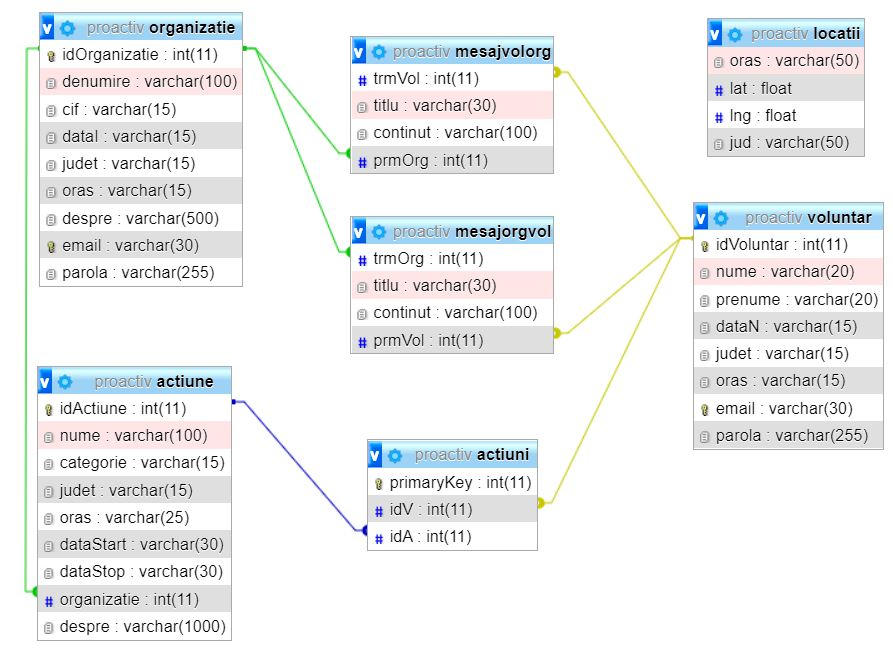
\includegraphics[width=0.8\linewidth]{./imagini/bazadate.jpg}
  \caption{Structura bazei de date a platformei Proactiv}
\end{figure}

\section{Tabele}
\par
Singurul tabel complet independent din baza de date “proactiv” este tabelul \textbf{locații}. Acesta cuprinde informații despre orașele importante din România, județul din care face parte fiecare în parte și coordonatele (latitudinea și longitudinea) la care sunt poziționate pe harta celor de la Google. Aceste informații sunt preluate din baza de date în momentul afișării acțiunilor de voluntariat pe hartă, pentru a poziționa fiecare pin la locația potrivită.
\\
\begin{figure}[H]
\centering
  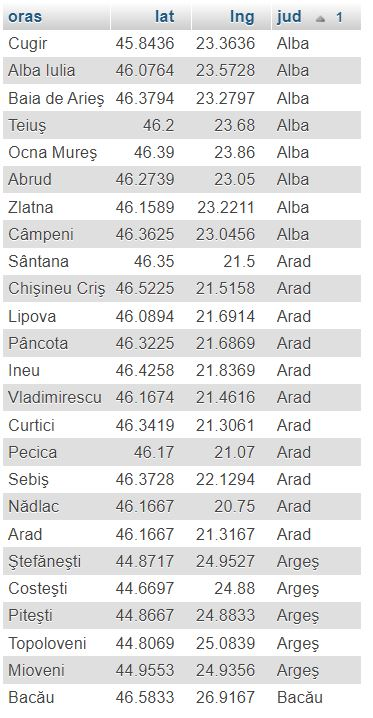
\includegraphics[width=0.6\linewidth]{./imagini/locatii.jpg}
  \caption{O mică parte din datele introduse în tabelul locații}
\end{figure}

\newpage
Tabelul \textbf{voluntar} stochează datele utilizatorului cu cont de tip voluntar, date introduse în momentul înregistrării pe platformă. Pe lângă aceste date preluate de la utilizator în momentul înregistrării, este alocată o cheie primară, unică și foarte importantă atât pentru funcționalitatea corectă a aplicației, cât și pentru logica structurii bazei de date.
\\
\begin{figure}[H]
\centering
  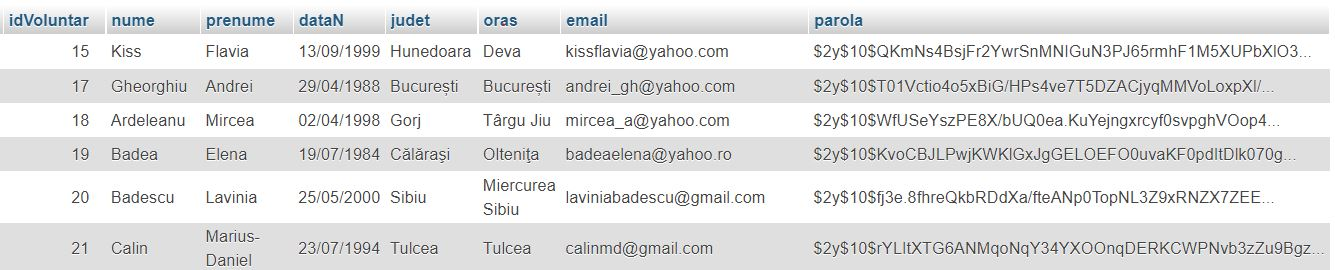
\includegraphics[width=1\linewidth]{./imagini/voluntar.jpg}
  \caption{Date introduse în tabelul voluntar}
\end{figure}
\par
Structura tabelului \textbf{organizație} este asemănătoare cu cea a tabelului descris anterior. Diferența este că acesta stochează datele utilizatorului cu cont de tip organizație, pentru care o parte din datele cerute diferă.
\\
\begin{figure}[H]
\centering
  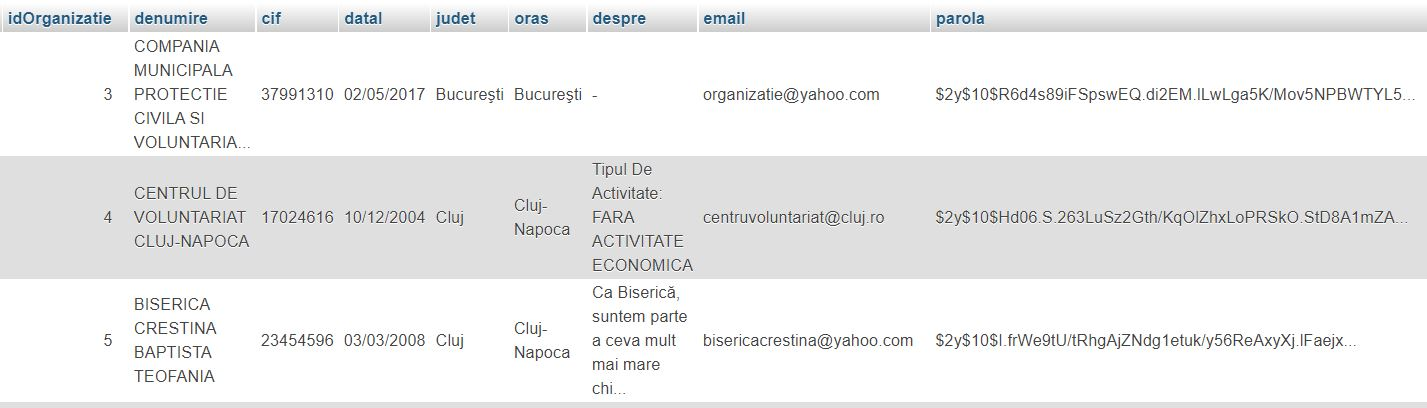
\includegraphics[width=1\linewidth]{./imagini/organizatie.jpg}
  \caption{Date introduse în tabelul organizație}
\end{figure}
\par
Pentru ambele tipuri de cont, parola este criptată în momentul adăugării contului nou în baza de date și decriptată în momentul în care se verifică corectitudinea acesteia pentru realizarea autentificării sau pentru actualizarea acesteia din pagina “Contul meu”.

\newpage
Tabelul \textbf{acțiune} stochează informațiile despre acțiunile semnalate de către utilizatorii cu cont de tip organizație. Pe lângă cheia primară și datele introduse de utilizator, pentru fiecare acțiune se stochează id-ul organizației care a semnalat-o, prin intermediul cheii străine cu numele “organizatie”.
\\
\begin{figure}[H]
\centering
  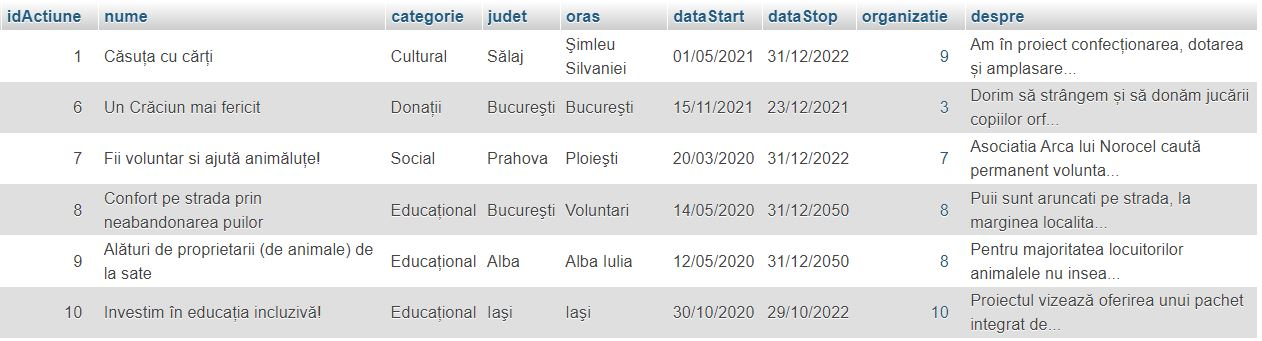
\includegraphics[width=1\linewidth]{./imagini/actiune.jpg}
  \caption{Date introduse în tabelul acțiune}
\end{figure}

\par
Tabelul \textbf{acțiuni} este podul de legătură dintre un anumit voluntar și o acțiune la care acesta a decis să se înscrie. Această legătură are loc prin utilizarea a două chei străine: idV, care face referință către cheia primară a voluntarului și una care face referință la id-ul unic al acțiunii, anume idA.
\\
\begin{figure}[H]
\centering
  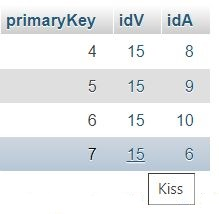
\includegraphics[width=0.4\linewidth]{./imagini/actiuni.jpg}
  \caption{Acțiunile la care este înscris voluntarul cu id-ul 15}
\end{figure}

\par
Tabelele \textbf{mesajorgvol} și \textbf{mesajvolorg} stochează mesajele trimise sau primite de către utilizatori. Acestea au drept coloane cheia primară a celui care a trimis mesajul, titlul mesajului, conținutul și cheia primară a celui care trebuie să primească mesajul trimis.


\chapter{Concluzii și direcții viitoare de dezvoltare}
\section{Concluzii}
\par
Lucrând pentru acest site web, am descoperit cât de mult îmi place domeniul programării web. Faptul că necesită imaginație, design-ul paginilor, alegerea paletelor potrivite de culori, schițarea unui logo, potrivirea elementelor pentru o experiență plăcută a utilizatorilor, dar și backend-ul și funcțiile scrise pentru a-i oferi platformei un scop și o funcționalitate, mă conving să mă apropi tot mai mult de acest domeniu și mă fac să îmi doresc să lucrez într-o companie care dezvoltă astfel de platforme web. 
\\ \par
O problemă întâmpinată în realizarea acestei lucrări a fost și, din păcate este în continuare, situația pandemică cu care ne confruntăm. Trecerea în online a îngreunat colaborarea cu profesorii, cu colegii și accesul la materiale utile în realizarea documentației. O altă problemă des întâlnită în cazul lucrărilor de licență tehnice, problemă întâmpinată și de mine, a fost cea a erorilor de cod. Cea din urmă problemă a prelungit finalizarea lucrării, dar a ajutat în acumularea de informații și cunoștiințe, din nevoia de a o rezolva.
\\ \par
Revenind la concluzii mai vesele, îmi place foarte mult gândul că orice modificare făcută în cod este la un refresh distanță, este vizuală, ușor de observat și de modificat în cazul în care nu este satisfăcătoare.



\section{Direcții viitoare}
\par
Planul meu este să îmbunătățesc această platformă web, puțin câte puțin, muncind să acumulez cunoștiințe și să mă perfecționez în acest domeniu.
\\ \par
Chiar îmi doresc să public site-ul Proactiv într-o zi, dar nu pentru profit sau pentru câștiguri financiare, ci deoarece cred cu adevărat că voluntariatul este un lucru foarte bun, altruist și satisfăcător sufletește, care merită promovat și încurajat în România.
\\ \par
Mi-ar aduce o satisfacție foarte mare gândul că, datorită mie și a platformei mele, mai mulți cetățeni au fost proactivi, mai multe organizații și-au găsit voluntarii de care aveau atât de multă nevoie și că mai multe persoane cu probleme sau dizabilități, animale neajutorate, familii sărace etc au fost ajutate și au un trai puțin mai decent.
\\
\begin{figure}[H]
\centering
  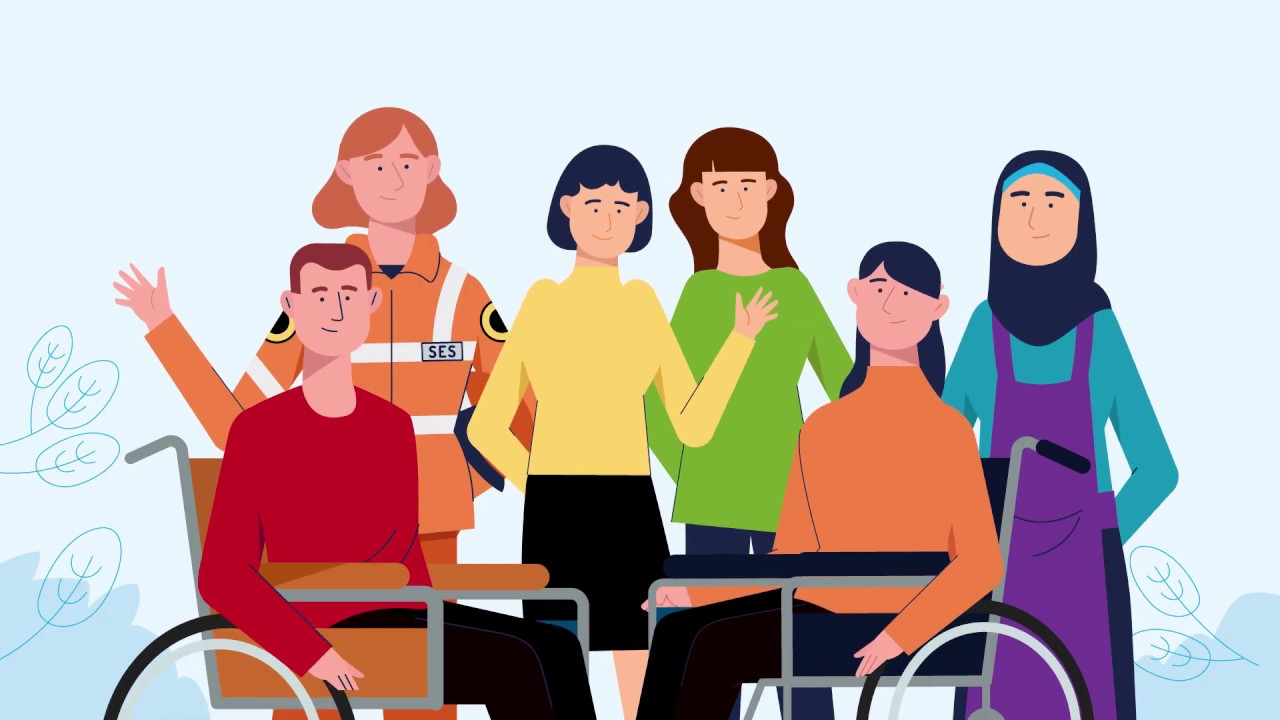
\includegraphics[width=1\linewidth]{./imagini/theend.jpg}
  \caption{Oamenii seamănă cu stâlpii de pe marginea drumului. Nu luminează decât dacă sunt legați între ei.}
\end{figure}


\begin{thebibliography}{1}
\bibitem{proactiv} 
Proactivitatea
\\\texttt{https://www.hipo.ro/locuri-de-munca/vizualizareArticol/578/Proactivitatea}

\bibitem{VBC} 
Roata Valorilor Voluntariatului
\\\texttt{https://volunteer.ca/index.php?MenuItemID=383}

\bibitem{greenr} 
Green Report
\\\texttt{https://green-report.ro/3-din-10-romani-fac-voluntariat/}

\bibitem{hv} 
Harta Voluntariatului
\\\texttt{https://hartavoluntariatului.ro}

\bibitem{dbv} 
De Bunavoie
\\\texttt{https://debunavoie.ro}

\bibitem{afg} 
All For Good
\\\texttt{https://www.allforgood.org/}

\bibitem{usecases} 
\textsc{Alistair Cockburn}, \emph{Writing Effective Use Cases}, Addison-Wesley Professional, 2000.

\bibitem{uml} 
\textsc{James Rumbaugh, Ivar Jacobson și Grady Booch}, \emph{The Unified Modeling Language Reference Manual 2nd Edition}, Addison-Wesley Professional, 2004.

\bibitem{gmaps} 
Google Maps API
\\\texttt{https://developers.google.com/maps/documentation/javascript/overview}

\bibitem{xampp} 
\textsc{Tom Butler}, \emph{Php \& Mysql: Novice To Ninja}, Site Point, 2017.

\end{thebibliography}
\addcontentsline{toc}{chapter}{Bibliografie}

\end{document} 